%% main_edit3.tex  -- REFRAME 3: CONSTRAINT-FIRST / MIP-CENTRED
%%
%% What changed from main_edit_rev2.tex and the earlier main_edit3 draft:
%%   - The generative-augmentation arm is removed from the design, the results,
%%     the notation and the appendices. The DATGAN route now appears only in the
%%     literature review, where it is the object of the argument in
%%     files/Introduction.tex: a generative model is fitted to the observed joint
%%     distribution, so the structural rules that make a record possible are not
%%     part of its objective; applications therefore repair the output, and once
%%     the rules must be written down rule by rule the constraint is doing the
%%     work. Construction inside the constraint set is adopted instead.
%%   - The pool stage is now (i) a CP feasible pool built from census conditionals
%%     under the 11 structural rules and (ii) mixed-integer pool expansion for
%%     zero-capacity cells. Household reconstruction and zone fitting are unchanged.
%%   - The results are a two-factor design: pool {raw microdata, CP feasible,
%%     CP feasible + MIP expansion} x fitter {SA, IPU, MIP}. Every arm carries a
%%     status column, and no arm is credited with a number it has not produced.
%%
%% CANONICAL BASES (unchanged from the previous revision):
%%   - 457 SA2 zones with complete control-table data; arm coverage differs.
%%   - donor for the raw microdata arms: 1,252,479 records (LINKED_DATA_clean.csv)
%%   - 11 control tables shared by all completed arms for the primary comparison
%%   - 353-zone cohort for the matched comparison; 213 zones for the audit
%%     (11 zones with CP-pool+SA)
%%
%% TODO(RUN) BEFORE SUBMISSION -- do not remove until each item is checked:
%%   [x] Batch the GAN stages out of the HPC submission flow (pbs/_gan_retired/);
%%       pbs/run_mip_expansion.pbs is the single submission for the MIP chain.
%% [x] Rebuild the CP feasible pool on the 11-table basis (2026-10-30):
%%       1,404,801 persons, 0 infeasible; coverage gap reduced to HRSP 101--103.
%%   [x] Ten-zone joint-marginal expansion audit (outputs/full10_joint_report.json):
%%       123 zero-capacity cells, 70 of 73 sourceable covered, 14 households.
%%   [ ] MIP-expanded pool + SA fit: not yet measured. The two rows in
%%       tab:pool_fitter_matrix are deliberately empty; do not fill them from
%%       another cohort.
%%   [ ] MIP-expanded pool + IPU fit: not yet measured, same condition.
%%   [ ] CP-pool+IPU on the 11 shared tables: populations exist
%%       (outputs/cp_ipu_results, 333 zone summaries) but only as a total RSSZ,
%%       so the arm cannot yet be placed beside the 11-table rows.
%%   [ ] Refit CP-pool+SA and CP-MIP on the rebuilt pool. BLOCKED, not merely
%%       pending: two harness defects must be fixed first, because a refit now
%%       reports a regression caused by the seeding, not the pool:
%%         (a) the 32 SA2s missing from csf_sa.csv inherit an SA3/SA4 REGUCP, so the
%%             pool slice for 112011236 is 34,632 persons against an 18,623 total;
%%         (b) calculate_total_marginals() returns 37,379 persons for that zone
%%             after normalize_counts() balances into the sexp 'Not applicable'
%%             bucket, i.e. the individual universe is roughly doubled.
%%       Measured cost: 18.8-33.7 min per zone locally, 1.14 h/zone on PBS, so the
%%       453-zone refit is ~21 days serial and must be submitted in chunks.
%%   [ ] Re-verify every number marked %% VERIFY against the canonical logs

\documentclass[review]{elsarticle}

\usepackage[margin=2.5cm]{geometry}

\usepackage[utf8]{inputenc}
\usepackage[dvipsnames]{xcolor}
\usepackage{keyz}
\usepackage{tikz}
\usepackage{censor}
\usepackage{tkz-graph}
\usepackage{booktabs}
\usepackage{blindtext}
\usepackage{graphicx}
\usepackage{filecontents}
\usepackage{subfiles}
\usepackage{tcolorbox}
\usepackage{pgffor}
\usepackage{subcaption}
\usetikzlibrary{shapes.geometric, arrows, positioning,fit, backgrounds,calc}
\usetikzlibrary{decorations.pathreplacing, decorations.markings}

%% Allow figure references from synth_pop outputs directories
\graphicspath{{./}{../synth_pop/outputs/benchmarking/}{../synth_pop/outputs/rssz_outlier/}{../synth_pop/outputs/paper_figures/}}

\tikzstyle{block} = [rectangle,draw,rounded corners,text width=6cm,align=center,fill=blue!10,line width=1pt]
\tikzstyle{blockd} = [diamond,draw,text width=2cm,align=center,fill=purple!10,line width=1pt]
\tikzstyle{arrow} = [thick,->,>=stealth,draw=blue]
\tikzstyle{title} = [font=\Large\bfseries,text centered]
\tikzstyle{VertexStyle} = [shape=rectangle,rounded corners,draw,minimum width=1.6cm,minimum height=0.8cm,align=center,font=\footnotesize]
\tikzstyle{EdgeStyle} = [->,>=stealth',line width=0.4pt,color=black!50]

\usepackage{amssymb}
\usepackage{amsmath}
\usepackage{hyperref}
\usepackage{glossaries}
\usepackage{cleveref}
\usepackage{algorithm}
\usepackage{catchfile}
\usepackage{algpseudocode}
\usepackage{placeins}
\usepackage{texosquery}
\usepackage{array}
\usepackage{expl3}
\usepackage{booktabs}
\usepackage{longtable}
\definecolor{ForestGreen}{rgb}{0.0, 0.258, 0.145}
\AtBeginDocument{\hypersetup{linkcolor=ForestGreen}}
\newif\ifstandalone
\standalonefalse

\makeatletter
\hypersetup{
    colorlinks=true,
    linkcolor=red,
    citecolor=red,
    filecolor=red,
    urlcolor=ForestGreen,
    linktoc=all
}
\makeatother

\begin{document}
\subfile{files/Acronymns}
\begin{frontmatter}

\author{Zeke Ahern\corref{cor1}\fnref{label1}}
\ead{z.ahern@qut.edu.au}

\title{Feasibility-Constrained Mixed-Integer Expansion of Candidate Pools for Synthetic Population Generation: Construction, Household Reconstruction, and Combinatorial Optimisation}

\affiliation[label1]{organization={School of Civil and Environmental Engineering, Queensland University of Technology},
           addressline={2 George St},
            city={Brisbane},
             postcode={4000},
              state={QLD},
              country={AU}}
\affiliation[label2]{organization={School of Mathematical Sciences, Queensland University of Technology},
           addressline={2 George St},
            city={Brisbane},
             postcode={4000},
              state={QLD},
              country={AU}}
\author{Helen Thompson \fnref{label2}}
\author{Alexander Paz\fnref{label1}}

\fntext[label1]{}
\fntext[label2]{}
\cortext[cor1]{}

\begin{abstract}
Zone-level synthetic population generation is limited less often by the fitting algorithm than by the candidate pool it draws from. Iterative proportional updating and simulated annealing can reweight and reselect the records they are given, but neither can produce a person whose attribute combination the pool does not contain, and a control table that requires such a cell cannot be matched by any weight vector. That support problem is treated here as the design object. The candidate pool is built by constraint-guided resampling from observed census conditionals under the eleven structural rules of the census dictionary, and where a zone's controls require a cell the pool cannot supply at all, a mixed-integer program adds the smallest set of rule-feasible donor--shell households that restores coverage, choosing them against every supplied marginal table at once. Because feasibility is established at construction, the pipeline carries no repair stage, and it is CPU-only and deterministic given a seed. The pipeline is applied to South-East Queensland and Tweed Heads (\textbf{457 SA2 zones}) using the \textbf{11 control tables shared by every completed arm}.

The design is a two-factor comparison: the pool is the raw microdata or the constructed feasible pool, with and without mixed-integer expansion, and the fitter is simulated annealing (SA), iterative proportional updating (IPU), or a tolerance-relaxed mixed-integer program (MIP). Three findings are reported. First, on the \textbf{11 control tables shared by every arm} and the \textbf{353 zones} with complete coverage, the constructed pool lowers SA's mean relative sum of squared z-scores from 0.416 to 0.205 and its median from 0.276 to 0.188, with IPU on the raw microdata at 0.376 and 0.250; a pool that is feasible by construction therefore helps a conventional fitter without any generative component. Second, feasibility of individual records does not imply exact zone-level fit: across the 453 fittable zones the mixed-integer fitter misses the worst cell of the median zone by a factor of 10.5 while its typical cell is off by 18\%, the best zone still misses its worst cell by 0.57, and no zone comes within 5\% on every cell, so a tolerance-relaxed program is a diagnostic instrument rather than a substitute for SA. Third, the expansion mechanism fills 70 of the 73 sourceable zero-capacity cells across ten audit zones with 14 households (18 persons), leaving uncovered only cells that the census extract cannot source. A cohort-matched audit shows no arm dominates: SA-Only attains the lowest mean joint total-variation distance (0.133, resolving four of eight designed pairs), the mixed-integer fit preserves pairwise association best (mean absolute Cram\'{e}r's $V$ difference 0.077) while duplicating 89.5\% of records within a zone, and CP-pool+SA carries the least cross-zone cloning (36.2\%) and the largest unseen share, with 86.9\% of its persons carrying a combination absent from the donor. The mixed-integer expansion of the fitted arms is specified, implemented and released but not yet measured on the full cohort; every row of the design table states its status, and code, control-table repairs and job logs are released so that each number here can be regenerated from a single run.
\end{abstract}

\end{frontmatter}

\subfile{files/Introduction}

\section{Methodology}
\label{sec:methodology}

\subsection{Problem Definition}
Population synthesis seeks a mechanism for generating detailed synthetic agents that reproduce the joint distribution and zone-level totals of an observed population. The recurring challenges are: (1) estimating the joint distribution $P(C_1,\dots,C_{n_c},D_1,\dots,D_{n_d})$ over continuous and discrete variables from a privacy-protected microsample; (2) preserving household relational structure; (3) reconciling many marginal control tables simultaneously; and (4) scaling to fine spatial resolution without losing fidelity. These challenges are well documented, and the techniques used to address them are well established. What is examined here is \emph{where feasibility enters the pipeline}. If it enters after the candidates have been proposed, the pipeline needs a repair stage, and the repair stage silently determines the output. If it enters at construction, every downstream stage operates on candidates that are already admissible and the fitting problem is purely one of allocation.

\subsection{Scope of the study}
\label{sec:contribution}
Each component of the pipeline---constraint-guided resampling from census conditionals, mixed-integer selection with forbidden-pair cuts, greedy household matching \citep{Gargiulo2010AnHouseholds}, and \gls{sa}/\gls{ipu} fitting \citep{Huang2001AMicrodata., Ye2009MethodologyPopulations}---is an established method. The work reported here has three parts:

\begin{enumerate}
    \item \textbf{An integrated, end-to-end pipeline} in which feasibility is a property of construction rather than of a post-processing stage: a cell-complete feasible pool is built directly from the census, expanded by a mixed-integer program where a zone requires a cell the pool cannot supply, grouped into households, and fitted by conventional \gls{sa} or \gls{ipu}.
    \item \textbf{A two-factor comparison design} spanning seven strategies (SA-Only, IPU-Only, CP-pool+SA, CP-pool+IPU, CP-MIP, and \gls{sa}/\gls{ipu} on the MIP-expanded pool) that separates the effects of the fitting algorithm from those of the candidate-pool construction. Every arm states the cohort it has completed on; an arm without a completed cohort carries no numbers.
    \item \textbf{A released, reproducible run}: a single pipeline run whose code, data-preparation decisions (including the repair of internally inconsistent census marginals), and job logs are released, so that the reported numbers can be traced and regenerated.
\end{enumerate}

What this study does \emph{not} establish is stated explicitly. In the pool comparison, pool size is confounded with pool composition, and the expanded-pool arms are a design whose pool-side mechanism has been audited on ten zones but whose fitted-zone metrics are not yet measured (Section~\ref{sec:benchmark}). The pool effect is therefore reported for the arms that have completed, and the expansion hypothesis is stated as a hypothesis rather than credited with any figure it has not produced.

\subsection{Strategy roles and expected benefits}
\label{sec:strategy_roles}
The combinations are designed to answer different questions; they are not expected to dominate on the same metric. The \emph{pool} determines which coherent person--household records are available, whereas the \emph{fitter} determines how those records are allocated to zones. Each comparison is therefore interpreted according to its intended benefit:

\begin{table}[htbp]
\centering
\caption{The component inventory from which a population is assembled, and the flag presets that define each synthesis arm. \textbf{Panel A} lists every module the released pipeline can switch on, in pipeline order; \textbf{Panel B} shows which modules each arm enables ($\bullet$ enabled, $\circ$ available but disabled). Expected benefits are hypotheses tested by the validation metrics, not assumptions that a method must outperform every other combination. \textsuperscript{\dag}Released and audited as a pool-construction step; its effect on the fitted-zone metrics is the experiment of Section~\ref{sec:benchmark} and is not yet measured.}
\label{tab:strategy_roles}
\footnotesize
\setlength{\tabcolsep}{4pt}
\emph{Panel A: components that can be combined}\\[1pt]
\begin{tabular}{@{}>{\raggedright\arraybackslash}p{2.2cm}>{\raggedright\arraybackslash}p{2.6cm}>{\raggedright\arraybackslash}p{10.2cm}@{}}
\toprule
\textbf{Stage} & \textbf{Flag} & \textbf{Mechanism, and what it contributes} \\
\midrule
Feasible pool & \texttt{-{}-cp-pool} & Constraint-guided donor resampling from observed census conditionals under the eleven structural rules. \emph{Gives} feasibility by construction, cell completeness over the modelled attributes, a CPU-only path, and no repair stage. \\
Pool expansion & \texttt{-{}-mip-expand} & Feasibility-constrained mixed-integer expansion over a donor--shell menu. A small set of rule-feasible records is selected against all supplied marginal tables simultaneously, with soft coverage of zero-capacity cells; no rule-infeasible combination is emitted and the full shortfall is not required. \emph{Adds} supported-but-unobserved records so pool coverage is less likely to bind the zone fit. \\
Household construction & \texttt{-{}-households} & Census-consistency rules plus greedy sequential matching (always enabled). \emph{Binds} individuals and dwelling terms into atomic household records. \\
Zone fitting & \texttt{-{}-fitter} \\texttt{\{ipu,sa,mip\}} & IPU weights, SA selection/swaps, or a tolerance-relaxed mixed-integer fit. \emph{Allocates} pool households to the zone-level control tables. \\
Validation & \texttt{-{}-validate} & Shared-11 RSSZ and marginal fit, pairwise Cram\'{e}r's $V$, and the unseen share. \emph{Keeps} pool and fitter effects separable. \\
\bottomrule
\end{tabular}
\\[4pt]
\emph{Panel B: arm presets over the same inventory}\\[1pt]
\begin{tabular}{@{}l*{3}{c}p{5.3cm}@{}}
\toprule
\textbf{Arm} & \texttt{cp} & \texttt{mip-exp} & \textbf{Fitter} & \textbf{Question the arm answers} \\
\midrule
SA-Only        & $\circ$ & $\circ$ & SA  & Baseline on the raw microdata \\
IPU-Only       & $\circ$ & $\circ$ & IPU & Weighting on the same restricted support \\
CP-pool+SA     & $\bullet$ & $\circ$ & SA  & Does a feasible pool help a conventional fitter? \\
CP-pool+IPU    & $\bullet$ & $\circ$ & IPU & Fitter contrast with the pool held fixed \\
CP-MIP         & $\bullet$ & $\circ$ & MIP & Exactness versus runtime and coverage \\
MIP+SA\textsuperscript{\dag} & $\bullet$ & $\bullet$ & SA  & Does restoring zero-cell coverage change the achievable fit? \\
MIP+IPU\textsuperscript{\dag} & $\bullet$ & $\bullet$ & IPU & Pool effect separated from the SA search \\
\bottomrule
\end{tabular}
\end{table}

The expected role of expansion is therefore \emph{support completion}, not automatic zone fitting. A useful expanded pool should make previously unavailable or rare combinations selectable while preserving household and cross-attribute relationships. If CP-pool+SA improves marginal fit but worsens joint or household metrics, the result is interpreted as a pool--fitter trade-off rather than a general improvement. If CP-MIP fits tolerance well but duplicates records within a zone, it demonstrates the cost of optimising feasibility rather than fidelity. If CP-pool+SA and CP-pool+IPU differ substantially, that difference is attributable to the fitter because their pool is held fixed. If expansion leaves the fitted metrics unchanged, the binding constraint was not pool support, and the honest conclusion is that the pool was already adequate.

Three implementation safeguards apply to the pool comparison. First, household construction precedes zone fitting: the solver selects whole linked households and never selects person rows independently after household IDs have been assigned. Second, every zone receives a status record containing dropped inconsistent households, unfillable control cells, saturated zero cells, solver failure reason, and whether an output was written. Third, the pool-side programs admit only combinations that satisfy the structural rule set, so a constraint violation in a released population is a defect of the implementation rather than a tolerated property of the method. These safeguards operationalise household-first expansion and systematic infeasibility reporting. A genuine joint State--SA4--SA2 objective remains a separate ablation: the current production results are SA2 fits and should not be described as multi-level.

\subsection{Constraint-first construction}
\label{sec:why_construction}
The design follows from the argument set out in Section~\ref{sec:bay}. A generative model is fitted to the observed joint distribution, and the structural rules that make a record admissible are not part of that distribution: they are prior knowledge, taken from the census dictionary, and they constrain combinations the microsample may not contain often enough to influence a loss function. Such a model can therefore emit records that are statistically plausible and logically impossible, and the applications that report violation rates handle them with a separate check-and-repair pass \citep{Kim2023ASynthesis}. Two consequences follow for this paper, and neither constitutes a claim about generative models in general. First, the repair pass is not a detail: if three quarters of candidate records require rewriting, the released population is the repaired sample, and the reported fidelity describes the repair as much as the model. Second, once the rules have been written down rule by rule and applied record by record, the constraint set is already the substantive object, and it can be enforced at construction instead. In this pipeline the feasible pool admits only combinations that satisfy the rule set, expansion adds only households that satisfy it, and there is no stage whose function is to undo another stage's output.

\subsection{Proposed Solution Methodology}
The production pipeline proceeds in five stages:

\begin{enumerate}
    \item \textbf{Feasible pool construction.} Attribute domains are taken from the ABS coding, the eleven census-consistency rules are expressed as explicit predicates, and the pool is assembled from observed census records together with structurally feasible but unobserved cells reconstructed by constraint-guided conditional resampling (Section~\ref{sec:cp}).
    \item \textbf{Pool expansion.} Where a zone's control tables require a control cell that the pool cannot supply at all, a mixed-integer program selects the smallest set of donor--shell households that restores coverage against all supplied marginal tables at once (Section~\ref{sec:mip_pool_expansion}).
    \item \textbf{Household reconstruction.} A greedy matching algorithm groups the pooled individuals into households (Section~\ref{sec:households}); expansion candidates already arrive as whole households.
    \item \textbf{Zone-level fitting.} \gls{ipu}, \gls{sa}, or a tolerance-relaxed mixed-integer fit draws households from the pool to match zone-level marginals (Section~\ref{sec:sa}).
    \item \textbf{Validation.} The result $T_\text{synth}$ is validated against the shared 11 census control tables (Section~\ref{sec:extval}).
\end{enumerate}

The comparison branches enter after pool construction. SA-Only and IPU-Only use
the raw microdata branch; CP-pool+SA, CP-pool+IPU and CP-MIP use the constructed
feasible pool; MIP+SA and MIP+IPU use that pool after expansion. Thus, a fitter
comparison must keep the pool fixed, while a pool comparison must keep household
reconstruction, controls, fitter, and validation fixed.

\paragraph{Component inventory and flag presets}
\Cref{tab:strategy_roles} states the inventory explicitly, because the integration
claim is easier to audit when the combinable parts are named. Each stage after the
data source is a module with a flag: the pool stage is \emph{additive}
(\texttt{-{}-cp-pool} and \texttt{-{}-mip-expand} can each be enabled, in that order),
household construction is always enabled, and the fitting stage is a \emph{selector}
over three implementations (\texttt{-{}-fitter ipu|sa|mip}). A synthesis arm is
therefore a flag preset over one shared implementation rather than a separate
program, which is what makes the comparisons matched: two arms differ only in the
flags that are set. Panel~B of \cref{tab:strategy_roles} gives the preset for every
arm reported here. Constructing a population for a new study is consequently a
matter of choosing the modules the available data support---feasible-pool construction
needs only the census and the zone control tables, and expansion needs the same
inputs---rather than of reimplementing the pipeline.

\subsection{Modelling Framework}
The pool is not the fitting method and cannot solve sparse or inconsistent margins by itself; it determines
which households are available for selection, and the fitter decides how often each is used.
The feasible pool anchors the candidate composition to observed census conditionals,
and the household constructor carries individual and dwelling-level terms together
into the zone-level fit. \gls{ipu} and \gls{sa} are therefore evaluated as
complementary fitting methods rather than as alternatives to pool construction, and
the mixed-integer fitter is evaluated as an exactness benchmark on the same pool.
A pool that is feasible by construction removes one failure mode---an output that
violates the rule set---but it does not determine the marginal fit, which remains
the fitter's objective and is measured separately below.

IPU is retained in the design for a reason that is easy to miss. It is the only
fitter here that changes weights and nothing else: it cannot add a record, invent
a category or repair a cell, so its residual error is bounded below by what the
pool contains. That makes it the cleanest test of whether the pool or the
allocation is binding, and it is why the design pairs it with both pools rather
than treating it as an also-ran. It is also the practical fitter for an expanded
pool: it has no solver, so the cost of fitting a 457-zone cohort is minutes rather
than days, and it inherits whatever support the pool has. Its known cost is that
person and household margins are weighted independently, so household totals can
drift; that is a property to measure, not a reason to exclude the arm.



\FloatBarrier
\subfile{files/formulation_edit2}

\section{Case Study}
\subsection{Data} \label{sec:casestudy}
The primary data source is the ABS 2021 Census. Microdata provides individual records at SA4 level (100{,}000--300{,}000 persons per region) to protect confidentiality; macrodata provides aggregated counts at SA2 level. The case study covers South-East Queensland and the Tweed (SA4 codes 301--319 and 112), where \textbf{457 SA2 zones} carry control-table data. Four of those zones have no individual target at all and are documented exclusions, which leaves \textbf{453 fittable zones}---the number the SA-Only and CP-pool+SA arms completed, and the number the MIP fitter solved once its extra zero-target output is set aside. The primary comparison uses only the \textbf{11 control tables carried by every completed arm}. The arms therefore overlap without being identical, so every comparison names its cohort and none mixes zone sets: \cref{tab:cohorts} is the single place where a cohort size is defined, and the text below refers to those names rather than to individual zone counts. For each category $m$ in control table $k$ and zone $z$, the census count is $E_{z,k,m}$ and the set of primary control tables is $\mathcal{K}_{11}$.

\begin{table}[h!]
\centering
\caption{Every cohort reported in this paper, with the arms that share it and the
metric computed on it. A zone count appearing anywhere in the results is one of
these rows; the rows differ because the arms completed on different zone sets and
because a metric needs only the tables its arms carry.}
\label{tab:cohorts}
\footnotesize
\setlength{\tabcolsep}{5pt}
\begin{tabular}{@{}lclp{7.0cm}@{}}
\toprule
\textbf{Cohort} & \textbf{Zones} & \textbf{Arms sharing it} & \textbf{What it is, and what it is used for} \\
\midrule
Scope            & 457 & all & SA2 zones with complete control-table data \\
Fittable         & 453 & SA-Only, CP-pool+SA, CP-MIP & Scope minus the four documented zero-target exclusions; mean and median RSSZ \\
CP-MIP output    & 454 & CP-MIP & The 453 fittable zones plus one excluded zone the solver fitted to four persons; tolerance basis \\
IPU              & 457 & IPU-Only & Weighting does not require the exclusions to be dropped; joint and marginal audit only \\
CP-pool+IPU      & 340, 295 & CP-pool+IPU & Populations written for 340 zones, of which 295 carry an RSSZ summary; no 11-table scoring yet \\
Primary 11 tables & 353 & SA-Only, IPU-Only, CP-pool+SA & Primary mean and median RSSZ comparison \\
Three-arm audit  & 213 & CP-MIP, IPU-Only, SA-Only & Diversity and association, 80 zones sampled per arm \\
Four-arm audit   & 11  & plus CP-pool+SA & The same metrics on a cohort CP-pool+SA reaches \\
Expansion audit  & 10  & expansion step & The capacity audit and the added records \\
\bottomrule
\end{tabular}
\end{table}

{\footnotesize\textit{Note:} the four exclusions are SA2s 304041102, 308051537, 310021279 and 311031315. 308051537 is the one that appears in the CP-MIP output, so 454 $+$ 3 accounts for the whole scope. The 340 and 295 figures for CP-pool+IPU are population files and summary rows respectively; the arm is built but not yet scored on the 11-table basis, so it carries no row in \cref{tab:pool_fitter_matrix}.}

\subsection{Experimental Settings}
\label{sec:expsettings}
The complete configuration is in the Supplementary Material. Key settings, all drawn from one production run: 1{,}252{,}479 ABS microdata records as donor material, of which 648{,}717 form the training-scale reference population used for household construction; 97 modelled attributes after dropping identifiers; \gls{sa} fitting with 1{,}000 iterations per zone, initial temperature $T_0=100$, cooling rate $\alpha=0.95$, RSSZ objective; CP pool construction from observed census conditionals with the eleven structural rules as predicates; expansion with a 64-household and 256-person budget per zone, coverage weight $\lambda_0=10^{5}$ and marginal weight $\lambda_1=10^{-2}$. The \textbf{fitting and primary scoring basis is the 11 shared control tables}. The fitting variants are each parallelised into 20 chunks and submitted as independent PBS jobs; walltime and exit codes are logged. The CP arms share a single constructed pool: CP-pool+SA applies the same SA sampler to it, CP-pool+IPU applies the same IPU implementation, and CP-MIP performs a tolerance-relaxed mixed-integer fit.

\subsubsection{Positioning against established synthesizers}
\label{sec:external_baselines}
The reviewer suggestion to compare against established synthesizers is important, but the
comparison must be made at the population-synthesis layer. ActivitySim is principally an
activity-based travel-demand simulator; its companion PopulationSim is the relevant
open-source population-synthesis baseline. POLARIS also couples population synthesis to
an integrated travel-demand model. Neither ActivitySim nor POLARIS should therefore be
treated as a black-box replacement for the present zone-fitting experiment.

The following external-baseline protocol is defined for a like-for-like comparison.
PopulationSim (and, where its data interface permits, the POLARIS population stage)
must receive the same seed households/persons, geography, 11 control tables, target
population, and random-seed policy as the proposed method. Each method must return
linked person and household tables. Every output is then scored on the same per-zone
marginal TVD and SRMSE, pairwise Cram\'{e}r's $V$ error, household consistency, unseen
share, and runtime measures. Failures to produce a zone are reported rather than
excluded. ActivitySim is evaluated only in a downstream utility test if activity
patterns are available; its behavioural simulation output is not counted as evidence
for demographic population-synthesis accuracy. This protocol prevents a difference in
travel-model assumptions, control coverage, or household identifiers from being
misreported as a pool-construction effect.

The established methods also suggest techniques that can be tested independently:
multi-level controls, entropy/list balancing with preservation of seed weights,
integerisation after fitting, and household-first expansion followed by person-level
consistency checks. The current pipeline already contains related components (IPU,
selection-only rebalancing in the CP route, and explicit integer household
construction), so these are included as ablations rather than as competing methods. In particular, an entropy/list-balancing ablation and a household-first
weighted expansion are higher-priority follow-ups than embedding ActivitySim's
behavioural model. No external-baseline result is claimed here until the same-input
protocol has been executed.

\subsection{Candidate-Pool and Household Construction}
\label{sec:pool_construction}

The candidate pool is built by \emph{feasibility-constrained construction} from the census rather than by sampling a fitted joint model: the constraint-programming (CP) feasible pool and its mixed-integer expansion are described in Section~\ref{sec:cp} and Section~\ref{sec:mip_pool_expansion}. This subsection describes how candidate records---whether observed microdata rows or constructed donor--shell records---are grouped into coherent households before zone-level fitting.

\subfile{files/mip_expansion_process}

\subsubsection{Reconstructing Households}
\label{sec:households}
Each candidate record carries household-level and individual-level attributes. A greedy sequential matching heuristic groups individuals into households; the algorithm and complexity analysis are in Appendix~\ref{sec:household_appendix}. Household reconstruction is emphasised as the least controlled stage of the pipeline: its output is not validated against a household-level ground truth beyond the size distribution implied by the census, and its downstream effect is treated as a limitation rather than a validated result.

Households are not formed the same way in every arm, so a household-level
score computed on one arm is not automatically comparable with the same score
on another (\cref{tab:hh_handling}). The two microdata arms carry the observed
ABS household identifiers, so every household they emit is a real census
household. The constructed arms keep the census shells and group only the
records that infill added; CP-MIP never groups anything at fit time because a
household is its decision variable, and expansion candidates arrive with their
dwelling terms already fixed by the shell they were built from.

The reconstruction is therefore an explicit step with its own error, and it
is measured on the household table released with the code (648{,}717
persons): it yields
308{,}522 households, of which 98.4\% match the stated dwelling size exactly
(99.3\% within one person; mean error 0.032) and 100\% agree internally on all
eight dwelling terms, while 98.6\% stay within a single SA2. Two structural
defects remain. Reconstructed households are too small---mean size 2.10
against 2.56 in the census microdata, with 44.0\% single-person households
against 27.0\%---and 17.1\% of the households containing a child under 15
contain nobody aged 15 or over, which is an unattended-minor household that
the census never records. These are errors of construction rather than of
fitting, and they motivate treating this stage as the least controlled part of
the pipeline rather than as a validated result. %% VERIFY: recomputed from
%% outputs/hh_match/cleaned_dataset_hhid.csv (post-repair, 2026-10-29).


\FloatBarrier

\subsubsection{Marginal-Table Repair}
\label{sec:pool_rebalance}
During validation an inconsistency was identified in the SDMX-derived rent and mortgage marginal tables: the rent table (RNTRD) counted approximately $2.8\times$ more rent-paying dwellings than the tenure tables (TEND, TENLLD) for the same zones, and both dollar-banded tables were truncated (rent bands above \$399/week and repayment bands above \$1{,}799/month absent from the live API). Fitting against mutually inconsistent margins is infeasible by construction. The two tables were repaired per zone by anchoring the rent-paying (respectively mortgage-paying) dwelling total to the tenure table and distributing it across the full band range according to the within-universe distribution in the microdata. The repair script and pre-repair originals are released with the code; this repair is a data-cleaning step, not a fitting procedure, and it is a precondition for every arm in the comparison rather than a property of any one of them.

\FloatBarrier

\begin{table}[h!]
\centering
\caption{How each arm obtains the household records it fits. The columns
state what enters the zone-level fit, what formed it, and the consequence for
household-level scoring. Only the reconstructed arms introduce a grouping
step; the others inherit households from the pool or treat the household as
the unit of fit.}
\label{tab:hh_handling}
\footnotesize
\setlength{\tabcolsep}{4pt}
\renewcommand{\arraystretch}{1.1}
\begin{tabular}{@{}>{\raggedright\arraybackslash}p{2.1cm}
                     >{\raggedright\arraybackslash}p{3.4cm}
                     >{\raggedright\arraybackslash}p{5.2cm}
                     >{\raggedright\arraybackslash}p{3.2cm}@{}}
\toprule
\textbf{Arm} & \textbf{Household unit} & \textbf{How it was formed} & \textbf{Consequence} \\
\midrule
SA-Only & Observed ABS households (1{,}252{,}479 records) & None: persons arrive already grouped, and SA adds, removes and swaps whole households & Household tables are fitted directly; every household emitted is a real census household \\
IPU-Only & Observed ABS households & None: person and dwelling margins are weighted independently of one another & Nothing ties a household's members to a common weight, so household totals drift downward \\
CP-pool+SA & Census household shells plus grouped infills & Census rows keep their \texttt{ABSHID}; infilled rows are grouped by household-attribute signature and cut to the stated dwelling size & The pool is feasible by construction, so no repair stage is needed and the shells are real dwellings \\
CP-pool+IPU & Census household shells plus grouped infills & Same pool and same shells as CP-pool+SA & Pool held fixed, so the difference from CP-pool+SA is the fitter \\
CP-MIP & One binary per candidate household & None at fit time: the household is the decision unit, so its members are selected together & Household atomicity is automatic; fitting adds no reconstruction error of its own \\
MIP+SA / MIP+IPU & Shell households plus expansion households & Expansion candidates are built on a real shell, so the added records arrive already atomic & The reconstruction error above is inherited, and expansion adds no new grouping step \\
\bottomrule
\end{tabular}
\end{table}

\subsection{Constraint-Programming Feasible Pool}
\label{sec:cp}
To separate \emph{how the candidate pool is built} from \emph{how it is fitted}, the CP pool is built directly from the census rather than sampled from a learned model: attribute domains are taken from the ABS coding, the same 11 census-consistency rules used throughout are expressed as explicit predicates, and the feasible cell space is the union of every observed census record and structurally feasible but unobserved cells reconstructed by constraint-guided conditional resampling from observed conditionals. The resulting pool is feasible by construction, cell-complete over the modelled attributes, deterministic given a seed, and requires neither a GPU nor a post-hoc repair step: the constraints are the method, not a cleanup stage. The rebuilt pool contains 1{,}404{,}801 persons with zero infeasible records; its only residual coverage gap is the hours-worked codes 101--103, which conflict with the age--hours rule store rather than being absent from the census. \Cref{fig:cp_pool} draws the step as a keep and an add rather than as a filter: the pool exceeds the extract because unobserved but rule-feasible combinations are written in alongside the observed records, not because records were removed.

\begin{figure}[t]
  \centering
  % Figure 1: raw microdata, CP enrichment, and targeted MIP pool expansion.
\providecolor{ForestGreen}{rgb}{0.0,0.258,0.145}
\resizebox{0.98\textwidth}{!}{%
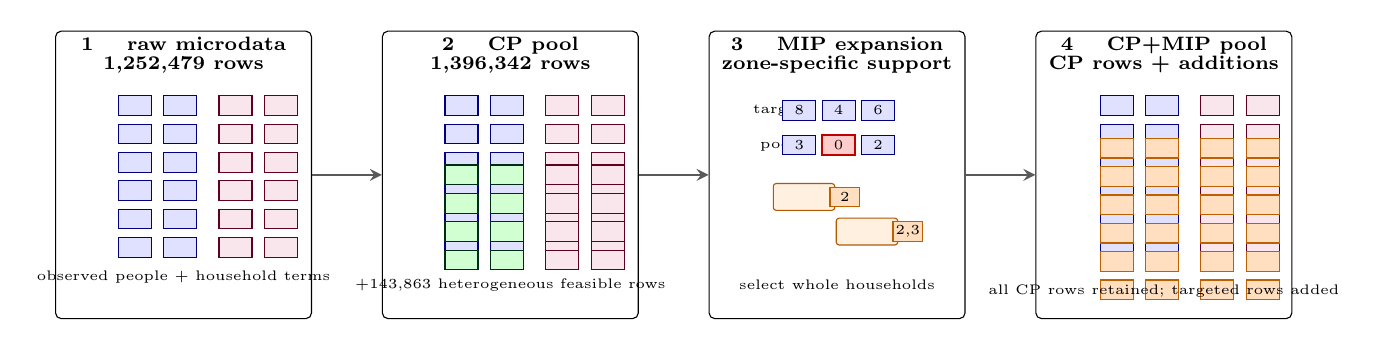
\begin{tikzpicture}[
  >=stealth,
  every node/.style={font=\small},
  panel/.style={draw, rounded corners=2pt, inner sep=5pt},
  title/.style={font=\scriptsize\bfseries, align=center},
  field/.style={draw, minimum width=0.42cm, minimum height=0.25cm,
                inner sep=0pt, align=center, font=\tiny},
  person/.style={field, fill=blue!12, draw=blue!50!black},
  household/.style={field, fill=purple!10, draw=purple!50!black},
  cpadd/.style={field, fill=green!18, draw=ForestGreen!65!black},
  mipadd/.style={field, fill=orange!25, draw=orange!75!black},
  zero/.style={field, fill=red!20, draw=red!75!black, line width=0.8pt},
  shell/.style={draw=black!65, rounded corners=1pt},
  arrow/.style={->, line width=0.9pt, draw=black!65}
]

% 1. Raw observed microdata.
\node[panel, minimum width=3.25cm, minimum height=3.65cm] (raw) at (0,0) {};
\node[title] at (0,1.52) {1 \quad raw microdata\\[-1pt]\scriptsize 1{,}252{,}479 rows};
\foreach \y in {0.88,0.52,0.16,-0.20,-0.56,-0.92} {
  \node[person] at (-0.62,\y) {};
  \node[person] at (-0.04,\y) {};
  \node[household] at (0.66,\y) {};
  \node[household] at (1.24,\y) {};
}
\node[font=\tiny] at (0,-1.30) {observed people + household terms};

% 2. CP construction adds broad feasible enrichment.
\node[panel, minimum width=3.25cm, minimum height=3.65cm] (cp) at (4.15,0) {};
\node[title] at (4.15,1.52) {2 \quad CP pool\\[-1pt]\scriptsize 1{,}396{,}342 rows};
\foreach \y in {0.88,0.52,0.16,-0.20,-0.56,-0.92} {
  \node[person] at (3.53,\y) {};
  \node[person] at (4.11,\y) {};
  \node[household] at (4.81,\y) {};
  \node[household] at (5.39,\y) {};
}
\foreach \y in {0.00,-0.36,-0.72,-1.08} {
  \node[cpadd] at (3.53,\y) {};
  \node[cpadd] at (4.11,\y) {};
  \node[household] at (4.81,\y) {};
  \node[household] at (5.39,\y) {};
}
\node[font=\tiny] at (4.15,-1.40) {+143{,}863 heterogeneous feasible rows};

% 3. MIP identifies a zone-specific support gap and candidate households.
\node[panel, minimum width=3.25cm, minimum height=3.65cm] (mip) at (8.30,0) {};
\node[title] at (8.30,1.52) {3 \quad MIP expansion\\[-1pt]\scriptsize zone-specific support};
\node[font=\tiny] at (7.55,0.82) {target};
\node[font=\tiny] at (7.55,0.38) {pool};
\foreach \x/\target/\cap in {7.82/8/3,8.32/4/0,8.82/6/2} {
  \node[person, minimum width=0.42cm] at (\x,0.82) {\target};
  \ifnum\cap=0
    \node[zero, minimum width=0.42cm] at (\x,0.38) {\cap};
  \else
    \node[person, minimum width=0.42cm] at (\x,0.38) {\cap};
  \fi
}
\node[shell, draw=orange!70!black, fill=orange!12,
      minimum width=0.78cm, minimum height=0.34cm, inner sep=0pt] at (7.88,-0.28) {};
\node[mipadd, minimum width=0.38cm] at (8.40,-0.28) {2};
\node[shell, draw=orange!70!black, fill=orange!12,
      minimum width=0.78cm, minimum height=0.34cm, inner sep=0pt] at (8.68,-0.72) {};
\node[mipadd, minimum width=0.38cm] at (9.20,-0.72) {2,3};
\node[font=\tiny] at (8.30,-1.40) {select whole households};

% 4. CP pool plus targeted MIP additions.
\node[panel, minimum width=3.25cm, minimum height=3.65cm] (expanded) at (12.45,0) {};
\node[title] at (12.45,1.52) {4 \quad CP+MIP pool\\[-1pt]\scriptsize CP rows + additions};
\foreach \y in {0.88,0.52,0.16,-0.20,-0.56,-0.92} {
  \node[person] at (11.85,\y) {};
  \node[person] at (12.43,\y) {};
  \node[household] at (13.13,\y) {};
  \node[household] at (13.71,\y) {};
}
\foreach \y in {0.34,-0.02,-0.38,-0.74,-1.10,-1.46} {
  \node[mipadd] at (11.85,\y) {};
  \node[mipadd] at (12.43,\y) {};
  \node[mipadd] at (13.13,\y) {};
  \node[mipadd] at (13.71,\y) {};
}
\node[font=\tiny] at (12.45,-1.48) {all CP rows retained; targeted rows added};

\draw[arrow] (raw.east) -- (cp.west);
\draw[arrow] (cp.east) -- (mip.west);
\draw[arrow] (mip.east) -- (expanded.west);

\end{tikzpicture}%
}

  \caption{How the two pool-construction stages differ. Constraint-guided programming
  (CP) broadly enriches the observed microdata with rule-feasible individual combinations,
  retaining the original records and shared household/dwelling terms. The MIP stage then
  audits a particular zone's pool slice, constructs feasible donor--shell households for
  zero-capacity cells, and appends only the selected targeted households. The final CP+MIP
  pool therefore contains broad CP enrichment plus targeted MIP additions; neither pool is
  yet a zone-level population.}
  \label{fig:cp_pool}
\end{figure}

The CP variants separate pool construction from fitting. \textbf{CP-pool+SA} applies the same SA sampler and iteration budget to the CP pool. \textbf{CP-pool+IPU} applies the same IPU implementation used by IPU-Only to that identical CP pool. The CP-SA versus CP-IPU contrast therefore measures the fitter while holding the candidate pool fixed; CP-IPU versus IPU-Only measures the value of a CP-feasible pool relative to raw microdata; and CP-pool+SA versus SA-Only measures the same pool effect under SA. \textbf{CP-MIP} selects households from the CP pool with a mixed-integer program and relaxes cell tolerances where exact zone-level margins are infeasible; its tolerance is therefore a fitted quantity, not a pass/fail threshold. Across the current CP-MIP run, 454 outputs contain at least one person: the 453 fittable zones plus SA2 308051537, one of the four documented zero-target exclusions, which the solver fitted to a four-person population. The remaining three exclusions have no output, so 454 plus 3 accounts for the whole 457-zone scope (\cref{tab:cohorts}). The CP path recombines observed conditional structure, so it is included to test whether a pool that is feasible by construction is sufficient for zone-level fidelity, and to establish that a rich candidate pool does not require a learned joint model.

A coding note that affects every arm. ABS QALFP (field of study) has sixteen two-digit categories: the twelve fields plus Mixed Field Programmes, and the supplementary codes for inadequately described, not stated, not applicable and overseas visitor. The fused microdata column carries fifteen, folding Mixed Field Programmes into ``inadequately described'', and its modal category sits at code 14 where the control tables place ``not applicable'' at 15. Applying the supplementary-code recode that the CP pool builder uses (codes $\ge 12$ shifted up one) reduces the SA-Only qalfp residual by a factor of 20 (0.1384 to 0.0070), which identifies the residual as a coding offset rather than a fit failure. Because the recode is applied inside the CP route and not to the raw-microdata arms, any qalfp comparison between CP and raw populations currently measures the recode; the released config exposes it as a single switch so that both bases can be reported.

\paragraph{MIP pool expansion}
\label{sec:mip_pool_expansion}
The constructed pool is feasible and cell-complete, but completeness is a
property of the pool, not of a zone: in a given zone a control-table cell
$(k,m)$ can require more records than that zone's slice of the pool can supply,
and in the limiting case no household in the slice carries the cell at all.
This is the zero-cell problem, and no weight vector or selection can repair it,
because the records needed do not exist. Expansion therefore treats the
zero-capacity case as the constraint it is, once the audit has established which
cells are in it.

\emph{What the audit measures.} For zone $z$ and control cell $(k,m)$, let
$E_{z,k,m}$ be the census target and $s_{z,k,m}$ the number of candidate records
in the zone's pool slice that carry the cell. The audit compares the target with
the \emph{attainable capacity} $r_{\max}s_{z,k,m}$, where $r_{\max}$ is the
largest number of times the zone fitter may replicate a single candidate, and
places every cell with $E_{z,k,m}>0$ in one of three states: \emph{sufficient}
if $r_{\max}s_{z,k,m}\ge E_{z,k,m}$; a \emph{partial shortfall} if
$0<r_{\max}s_{z,k,m}<E_{z,k,m}$, which replication can reach and which is
therefore left to the fitter; and \emph{zero capacity} if $s_{z,k,m}=0$, which
no weight, selection or replication can reach because the candidates are absent.
Only the third state is a pool deficiency, and only the third state is what
expansion addresses. The distinction matters for how a poor zone fit is read: a
cell in the second state is a fitting outcome, a cell in the third is a support
defect that no fitter could have avoided, and the two are reported separately
rather than pooled into one error term. \Cref{fig:mip_expansion} follows one zone
through the step, and Table~\ref{tab:cp_vs_mip} states how construction and
expansion differ.

\begin{figure}[t]
  \centering
  % =============================================================================
% fig:mip_expansion -- filling a zone's zero-capacity cells.
%
% Same board language as fig:cp_pool, one zone wide: a zone's control board has
% a positive target in a square its pool slice cannot supply at all, and no
% weight vector, selection or replication can reach it. Expansion builds
% donor x shell candidates for exactly those squares, one program per zone
% selects a handful, and the board is complete.
%
% Square states: blue = the pool slice covers the target; amber = covered but
% short; red = a positive target with no supply.
%
% Editing rules: no \\ inside a braced group; keep card text short, because the
% board is only ~2 cm tall and the cards sit beside it.
% =============================================================================
\providecolor{ForestGreen}{rgb}{0.0,0.258,0.145}
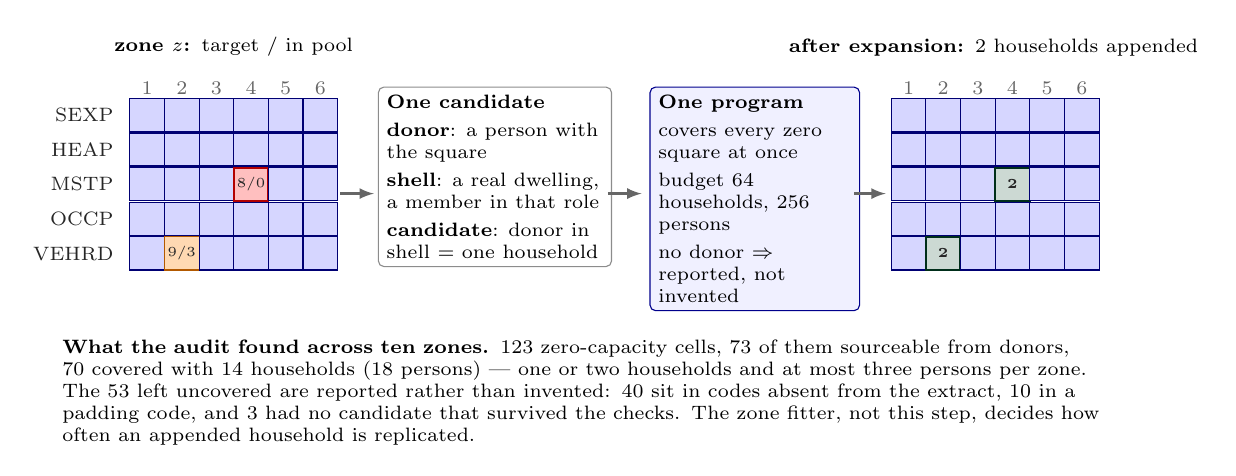
\begin{tikzpicture}[
  font=\footnotesize,
  >=latex,
  sq/.style={draw=black!50, minimum width=0.44cm, minimum height=0.42cm,
             inner sep=0pt, line width=0.4pt},
  have/.style={sq, fill=blue!16, draw=blue!45!black},
  short/.style={sq, fill=orange!30, draw=orange!70!black},
  zero/.style={sq, fill=red!25, draw=red!70!black, line width=0.8pt},
  filled/.style={sq, fill=ForestGreen!20, draw=ForestGreen!70!black, line width=0.8pt},
  hdr/.style={font=\scriptsize, text=black!60, inner sep=1pt},
  rowlab/.style={font=\scriptsize, anchor=east, text=black!85, inner sep=2pt},
  tag/.style={font=\scriptsize, text=black!75, align=center, inner sep=2pt},
  flow/.style={->, thick, draw=black!60},
  card/.style={draw=black!45, rounded corners=2pt, align=left, inner sep=3pt,
               fill=white},
  val/.style={font=\tiny, text=black!85, inner sep=0pt},
]

% ============================================================ board, zone z
\node[font=\scriptsize\bfseries, anchor=south] at (2.27,0.62)
  {zone $z$: \textnormal{target / in pool}};

\foreach \c [count=\j] in {1,...,6} {
  \node[hdr] at ({0.95+(\j-0.5)*0.44},0.34) {\c};
}

% 1 = covered, 0 = covered but short, 2 = no supply at all.
\foreach \r/\row/\name in {%
  0/{1,1,1,1,1,1}/SEXP,%
  1/{1,1,1,1,1,1}/HEAP,%
  2/{1,1,1,2,1,1}/MSTP,%
  3/{1,1,1,1,1,1}/OCCP,%
  4/{1,0,1,1,1,1}/VEHRD}%
{
  \node[rowlab] at (0.82,{-\r*0.44}) {\name};
  \foreach \d [count=\j] in \row {
    \pgfmathsetmacro{\x}{0.95+(\j-0.5)*0.44}
    \pgfmathsetmacro{\y}{-\r*0.44}
    \ifnum\d=2
      \node[zero, label={[val]center:8/0}] at (\x,\y) {};
    \else\ifnum\d=0
      \node[short, label={[val]center:9/3}] at (\x,\y) {};
    \else
      \node[have] at (\x,\y) {};
    \fi\fi
  }
}

% ======================================================== candidate for a cell
\draw[flow] (3.62,-1.00) -- (4.05,-1.00);

\node[card, anchor=north west] (cand) at (4.10,0.36) {\parbox{2.75cm}{%
  \scriptsize\raggedright
  \textbf{One candidate}\\[2pt]
  \textbf{donor}: a person with the square\\[2pt]
  \textbf{shell}: a real dwelling, a member in that role\\[2pt]
  \textbf{candidate}: donor in shell $=$ one household}};

% ================================================================ one program
\draw[flow] (7.02,-1.00) -- (7.45,-1.00);

\node[card, draw=blue!55!black, fill=blue!6, anchor=north west, name=prog]
  at (7.55,0.36)
  {\parbox{2.45cm}{\scriptsize\raggedright
  \textbf{One program}\\[2pt]
  covers every zero square at once\\[2pt]
  budget 64 households, 256 persons\\[2pt]
  no donor $\Rightarrow$ reported, not invented}};

% ==================================================================== settled
\draw[flow] (10.15,-1.00) -- (10.55,-1.00);

\node[font=\scriptsize\bfseries, anchor=south] at (11.92,0.62)
  {after expansion: \textnormal{2 households appended}};

\foreach \c [count=\j] in {1,...,6} {
  \node[hdr] at ({10.62+(\j-0.5)*0.44},0.34) {\c};
}

\foreach \r/\row/\name in {%
  0/{1,1,1,1,1,1}/SEXP,%
  1/{1,1,1,1,1,1}/HEAP,%
  2/{1,1,1,3,1,1}/MSTP,%
  3/{1,1,1,1,1,1}/OCCP,%
  4/{1,3,1,1,1,1}/VEHRD}%
{
  \foreach \d [count=\j] in \row {
    \pgfmathsetmacro{\x}{10.62+(\j-0.5)*0.44}
    \pgfmathsetmacro{\y}{-\r*0.44}
    \ifnum\d=3
      \node[filled, label={[val]center:\textbf{2}}] at (\x,\y) {};
    \else
      \node[have] at (\x,\y) {};
    \fi
  }
}

% ================================================================ audit line
% Anchored below the tallest card rather than at a fixed y, so the note cannot
% collide with the card text when the wording changes.
\node[anchor=north west, align=left, text width=13.2cm, font=\scriptsize,
      inner sep=1pt] at ($(prog.south west)+(-7.50,-0.32)$)
  {\textbf{What the audit found across ten zones.} 123 zero-capacity cells, 73 of
   them sourceable from donors, 70 covered with 14 households (18 persons) --- one
   or two households and at most three persons per zone. The 53 left uncovered are
   reported rather than invented: 40 sit in codes absent from the extract, 10 in a
   padding code, and 3 had no candidate that survived the checks. The zone fitter,
   not this step, decides how often an appended household is replicated.};

\end{tikzpicture}

  \caption{How a zone's zero-capacity cells are filled. For each zone the audit compares
  every positive-target cell with the supply in that zone's pool slice; on the board, a
  filled square is a cell the slice covers, an amber square one it covers only partly, and
  a red square one it cannot supply at all. A square with no supply cannot be reached by
  any weight vector, selection or replication. Each such cell
  receives a candidate: a real donor who carries the cell, written into a real shell
  dwelling from the same region that already has a member in the donor's role, so the
  dwelling and family terms stay observed rather than invented. One program per zone then
  selects a small set of candidates covering all zero cells at once, and the selected
  households are appended to the pool with fresh identifiers. Coverage is soft: a cell with
  no donor anywhere is reported by the audit rather than synthesised, and the zone fitter
  (IPU, SA or MIP), not this step, decides how often an appended household is replicated.}
  \label{fig:mip_expansion}
\end{figure}


\begin{table}[h!]
\centering
\caption{The two pool-side programs answer different questions and are not
substitutes. Construction makes the pool complete over the modelled attributes for
every zone at once; expansion repairs the cells a single zone's slice cannot supply.
Neither stage allocates records to zones, which is why both are followed by a fitter.}
\label{tab:cp_vs_mip}
\footnotesize
\setlength{\tabcolsep}{5pt}
\begin{tabular}{@{}>{\raggedright\arraybackslash}p{1.7cm}
                 >{\raggedright\arraybackslash}p{5.6cm}
                 >{\raggedright\arraybackslash}p{6.3cm}@{}}
\toprule
 & \textbf{CP pool construction} & \textbf{MIP pool expansion} \\
\midrule
Question & Can every rule-feasible cell be represented in the pool at all? &
Which cells can this zone's slice not supply, and which households can fill them? \\
Scope & The whole census, all zones at once, all 19 control tables &
One zone, and only the cells the audit places in the zero-capacity state \\
Decision & Which category each modelled attribute takes, given a household shell and the
observed conditional distributions & Which candidates enter a small added set, one binary
per candidate, against all marginal tables at once \\
Guarantee & Every emitted record satisfies $\mathcal{R}$, and the pool is cell-complete
over the modelled attributes & Every added household satisfies $\mathcal{R}$, and every
sourceable zero cell receives at least one candidate \\
Does not & Use zone targets, match any zone total, or decide replication & Close the
zone's full deficit, fit its totals, or decide how often a candidate is used \\
Cost & 27.1 minutes and 5.0\,GB for the whole pool, once & About 100 seconds per zone,
and only where zero cells exist \\
Result here & 1{,}404{,}801 persons, no rule violations & 14 households (18 persons)
across the ten audit zones \\
\bottomrule
\end{tabular}
\end{table}

\emph{Candidate construction.} For a zone $z$ let $\mathcal{Z}_z^0$ be the set of
control cells with a positive census target and zero attainable capacity in the
zone's candidate pool. For each such cell the module draws donor records from the
census microdata that carry the cell, pairs each donor member profile with a real
shell household from the same \texttt{REGUCP} that has a member in the donor's
\texttt{RLHP} role, and writes the donor profile into that slot. If the donor
profile conflicts with the shell's dwelling terms or with the rule set
$\mathcal{R}$, a small completion program finds the closest feasible profile,
\begin{equation}
\min_{y}\;\sum_{a}\bigl(1-y_{a,\tau(a)}\bigr)
\quad\text{s.t.}\quad
\sum_{c} y_{a,c}=1,\;\;
y_{a_1,c_1}+y_{a_2,c_2}\le 1 \;\;\forall\,(a_1,c_1,a_2,c_2)\in\mathcal{C},
\label{eq:mip_repair}
\end{equation}
where $\tau(a)$ is the donor's code for attribute $a$ and $\mathcal{C}$ is the
set of forbidden category pairs obtained by evaluating the shared rule set over
every attribute domain mesh (2{,}027 cuts in the ten-zone development audit).
Equation~\eqref{eq:mip_repair} is a \emph{candidate repair}, not the pool
objective: it preserves a real donor profile wherever the hard rules allow, and
it is solved separately for each candidate before any selection. The
household-level fields are fixed to the shell, so every candidate remains atomic
and family-coherent; candidates that fail the shared
rule checks are discarded, never patched. For attributes outside
the person-level model (e.g.\ \texttt{tend}, \texttt{typp}, \texttt{indp},
\texttt{stup}, \texttt{assnp}), a person-level repair is not available, so the
module falls back to a whole real donor household copied verbatim; the observed
household is feasible by construction.

\emph{Joint-marginal selection.} The candidates are then selected together, not
cell by cell. Let $\mathcal{J}_z$ index the candidate households,
$x_j\in\{0,1\}$ indicate selection, and $s_j$ be the number of persons in
candidate $j$. For a control cell $(k,m)$, let $a_{j,k,m}$ be the candidate's
contribution---the number of its members in the cell for a person-level table, or
one if the household sits in the cell for a household-level table---and let
$u_{j,k}=s_j$ for a person-level table and $u_{j,k}=1$ for a household-level
table. With the zone target $E_{z,k,m}$ and target share
\begin{equation}
q_{k,m}=\frac{E_{z,k,m}}{\sum_{m'\in\mathcal{M}_k}E_{z,k,m'}},
\label{eq:mip_share}
\end{equation}
the selection program is
\begin{equation}
\begin{aligned}
\min_{x,e,d}\quad &
\lambda_0\sum_{c\in\mathcal{Z}_z^0} e_c
\;+\;\sum_{k\in\mathcal{K}}\sum_{m\in\mathcal{M}_k} w_{k,m}\,d_{k,m}
\;+\;\lambda_1\sum_{j\in\mathcal{J}_z} x_j \\
\text{s.t.}\quad &
\sum_{j\in\mathcal{J}_z} a_{j,c}\,x_j+e_c\ge 1,
&& c\in\mathcal{Z}_z^0,\\
& d_{k,m}\ge \sum_{j\in\mathcal{J}_z}
  \bigl(a_{j,k,m}-q_{k,m}u_{j,k}\bigr)x_j,
&& k\in\mathcal{K},\,m\in\mathcal{M}_k,\\
& d_{k,m}\ge -\sum_{j\in\mathcal{J}_z}
  \bigl(a_{j,k,m}-q_{k,m}u_{j,k}\bigr)x_j,
&& k\in\mathcal{K},\,m\in\mathcal{M}_k,\\
& \sum_{j\in\mathcal{J}_z}x_j\le K_z,\qquad
  \sum_{j\in\mathcal{J}_z}s_jx_j\le P_z^{\mathrm{add}},\\
& \sum_{j\in\mathcal{J}_z(h)}x_j\le 1,
&& h\in\mathcal{H}_z,\\
& x_j\in\{0,1\},\quad e_c\ge 0,\quad d_{k,m}\ge 0.
\end{aligned}
\label{eq:mip_joint}
\end{equation}
Here $w_{k,m}=1/(|\mathcal{M}_k|\max(E_{z,k,m},1))$ gives every control table
equal weight and prevents large person tables from dominating; the
implementation divides $w$ by its maximum, a positive rescaling that does not
change the argmin. The released defaults are $\lambda_0=10^5$ and
$\lambda_1=10^{-2}$. With the default 256-person budget the whole marginal term
is below about $2.6\times10^4$, so covering one zero cell is worth more than
any marginal improvement the added set can buy. Coverage is still soft: an
unsourceable cell cannot make the program infeasible, and a cell can be left
uncovered when the budget or the candidate menu makes coverage impossible.
$K_z$ and $P_z^{\mathrm{add}}$ are small budgets (defaults: 64 households and
256 persons per zone), not the zone's population. The constraint over
$\mathcal{J}_z(h)\subseteq\mathcal{J}_z$ permits at most one transplant per
shell household.

The important difference from a per-cell objective is that
\eqref{eq:mip_joint} uses \emph{one} selection vector $x$ for \emph{all} control
tables. The deviations $d_{k,m}$ are therefore not independent cell repairs:
they measure how far the selected agents' aggregate profile is from the zone's
total marginal composition, table by table, and the solver must trade those
deviations against one another and against coverage. A set of records that fills
every zero cell but distorts the income or tenure shares is penalised; a set that
matches the shares but leaves a zero cell uncovered is penalised more heavily
through $\lambda_0$. This is a joint fit over the marginal tables, not a fit to
the full joint distribution: one selection vector must satisfy every table
simultaneously, while the joint distribution over attribute combinations is the
object of the zone fitter, not of the small pool-expansion program. The
coverage constraints are soft ($e_c$) precisely so that an unsourceable
cell---a structural zero, a padding code, or a cell with no donor anywhere---does
not make the program infeasible; it is reported instead.

The model is deliberately \emph{not} required to close the measured shortfall.
The deficit in a zone is often tens of thousands of persons, while the candidate
pool is a 5\% microsample and the added set is a few dozen households. Requiring
$\sum_j a_{j,k,m}x_j\ge E_{z,k,m}$ for every cell would either be infeasible or
force the pool to replicate the census many times over, which is the fitter's
job, not the pool's. What the expansion asks for is weaker and sufficient:
\emph{every zero cell for which a candidate exists should receive at least one
feasible candidate}, and the added candidates should jointly resemble the zone's
marginal totals. Because coverage is soft, a cell can still be left uncovered
when the budget or the candidate menu makes coverage impossible; such cells are
reported rather than silently dropped. The zone fit that follows decides which
candidates are actually used.

The module reports, per zone, the number of zero-capacity cells, how many are
covered, the selected household and person counts, the weighted joint-marginal
deviation, and the uncovered cells; the candidate-skip reasons are aggregated
over the run.

\emph{Development audit.} A ten-zone audit at the released defaults found 123
zero-capacity cells among 146 deficient cells (the other 23 were partial
shortfalls left to the zone fitter). The module generated donor--shell
candidates for 70 of the 73 sourceable zero cells and the joint selection
covered all 70, using 14 households (18 person rows) in total---one or two
households and at most three persons per zone, far inside the 64-household and
256-person budgets. All ten selection programs solved to optimality, and every
selected row passed the 11 shared rule checks. The 53 cells
left uncovered were 40 cells in four control codes absent from the census
extract, 10 \texttt{tend:6} padding cells, and three \texttt{tenlld:11} cases where no
donor--shell candidate survived the household and rule checks. The weighted
joint-marginal deviation of the added set was 0.239--1.622 per zone (median
0.406), and its unweighted mean absolute cell deviation was 0.126--0.280. These
are deviations of the added set, not of the fitted zone population; the audit
establishes that the mechanism can fill the sourceable zero cells with a small
number of feasible records, not that it closes the zone's full deficit.
Appendix~\ref{sec:pool_expansion_audit} gives the per-zone table and the
interpretation of the residual cells.
%% Audit source: outputs/full10_joint_report.json and
%% outputs/full10_joint_audit.log (10 zones, joint mode, released defaults;
%% 1,013.5 s).


\subsection{Benchmark Analysis}
\label{sec:benchmark}
The comparison design is two-factor. The pool is the raw microdata (SA-Only, IPU-Only), the constructed feasible pool (CP-pool+SA, CP-pool+IPU), or the constructed pool with mixed-integer expansion (MIP+SA, MIP+IPU); the fitter is \gls{sa}, \gls{ipu}, or the tolerance-relaxed MIP (CP-MIP). \Cref{tab:pool_fitter_matrix} states, for each of the seven arms, the cohort on which it has completed and the metric basis, so that no arm is credited with a number it has not produced. SA-Only and IPU-Only are the fixed-support controls; CP-pool+SA isolates the pool effect under a fixed fitter; CP-pool+IPU isolates the fitter under a fixed pool; CP-MIP tests what feasibility buys when it is optimised directly; and the two expanded-pool arms are the experiment on which the paper's pool-side argument rests.

\begin{table}[h!]
\centering
\caption{The pool $\times$ fitter design, with the completion status of each arm. Mean and median RSSZ are reported on the \textbf{11 control tables shared by every arm} over the \textbf{353 zones} with complete coverage of those tables; smaller is better. RSSZ is the primary objective for SA, but it can also be calculated post hoc for IPU and CP-MIP. CP-MIP minimises cell tolerance rather than RSSZ, so its post-fit RSSZ is a diagnostic rather than an optimisation result and is marked pending until the completed populations are rescored.}
\label{tab:pool_fitter_matrix}
\footnotesize
\setlength{\tabcolsep}{4pt}
\begin{tabular}{@{}lllcccp{4.6cm}@{}}
\toprule
\textbf{Arm} & \textbf{Pool} & \textbf{Fitter} & \textbf{Zones} & \textbf{Mean} & \textbf{Median} & \textbf{Status} \\
\midrule
SA-Only      & raw microdata & SA  & 353 & 0.416 & 0.276 & Complete on the 11 shared tables \\
IPU-Only     & raw microdata & IPU & 353 & 0.376 & 0.250 & Complete on the 11 shared tables \\
CP-pool+SA   & CP feasible   & SA  & 353 & \textbf{0.205} & \textbf{0.188} & Complete on the 11 shared tables \\
CP-pool+IPU  & CP feasible   & IPU & --- & --- & --- & Built (340 populations); no 11-table scoring \\
CP-MIP       & CP feasible   & MIP & 353 & --- & --- & Post-fit 11-table RSSZ pending; minimax cell error is the optimisation objective \\
MIP+SA       & CP + expansion & SA & --- & --- & --- & Pool audited on 10 zones; fit not run \\
MIP+IPU      & CP + expansion & IPU & --- & --- & --- & Pool audited on 10 zones; fit not run \\
\bottomrule
\end{tabular}
\end{table}
{\footnotesize\textit{Note:} the 11 shared tables are the control tables carried by every completed arm (heap, mstp, mtwp, occp, rlhp, sexp, hind, mrerd, nprd, rntrd, vehrd). RSSZ is optimised by SA, while IPU and CP-MIP can be rescored against the same 11-table basis after fitting; such a value measures realised marginal error but does not imply that the fitter optimised RSSZ. CP-MIP now minimises the worst relative cell deviation, protecting individual cells from being sacrificed to a weighted aggregate objective. Its RSSZ remains a post-fit diagnostic, reserved for the 353-zone common cohort. The two expanded-pool rows are deliberately empty: the expansion mechanism has been audited as a pool-construction step (Section~\ref{sec:mip_pool_expansion}) but the zone fits that would fill them have not been run, and the refit is blocked by a seeding defect described in the released run notes, so a number there would come from a different cohort or a defective harness.}

\textbf{The pool effect on a conventional fitter.} On the primary 11-table basis, mean RSSZ is reduced by 51\% by CP-pool+SA relative to SA-Only (0.205 against 0.416) and the median by 32\% (0.188 against 0.276), with every zone drawn from the same 353-zone cohort and every table from the same 11-table set. The improvement is therefore attributable to the candidate pool: the fitter, its iteration budget, its temperature schedule and its acceptance rule are identical in the two arms, and the only difference is whether the records were drawn from the raw microdata or constructed under the rule set. Two mechanisms are consistent with the size of the gain. The constructed pool is cell-complete over the modelled attributes, so a category that the 5\% microsample happens to miss in a zone is still selectable; and it is not confined to joint combinations the microsample contains, so a zone whose household-level marginals require an archetype absent from the sample is no longer forced to accept the nearest available real household. It is noted that the pool also differs in size (1{,}404{,}801 records against 1{,}252{,}479), so this comparison identifies the constructed pool as a whole, not the feasibility property alone.

\textbf{Fitter contrast under a fixed pool.} CP-MIP shows what optimising feasibility directly achieves, and the answer is a caution. Across the 453 fittable zones the worst cell of the median zone misses its target by a factor of 10.5 (interquartile range 7.0--15.1 across zones) and that of the best zone by 0.57, while the typical cell misses by 18\%: no zone comes within 5\% on every cell. The typical cell is therefore close and a small number of cells with small targets set the tolerance, which is what a mutually inconsistent control set looks like once it is solved exactly rather than weighted. Feasibility of individual records at pool construction therefore does not imply exact zone-level marginal fit after fitting: the mixed-integer program finds a feasible selection, but the control tables it must satisfy simultaneously are mutually inconsistent at zone level, so the tolerance relaxation---not the solver---determines the outcome. This is the reason the mixed-integer route is reported as a diagnostic instrument and as a pool-construction tool rather than as a replacement for SA.

\textbf{What the expanded-pool arms test.} The expansion argument is a claim about a specific failure mode: a control cell with a positive target and zero attainable capacity in the zone's pool cannot be matched by any weight vector or selection, because no candidate carries the cell. Removing that blockage is a necessary condition for the fitter to reach the cell, and it is not a claim that the fit is otherwise improved. The mechanism audit in Section~\ref{sec:mip_pool_expansion} establishes that the blockage can be removed with a handful of feasible households. Whether the fitted metrics move is a separate question, and it is the one the two empty rows are reserved for.

Some results remain weak for particular attributes and sparse zones. Those failures are
reported rather than hidden: the benchmark tables retain per-table and per-zone
distributions, and the interpretation distinguishes (i) candidate-pool coverage,
(ii) household reconstruction consistency, and (iii) zone-level optimisation. A good
association score does not compensate for poor household totals or a large RSSZ in a
sparse zone, and no component is described as a universal solution.

\gls{ipu} optimises weights independently at individual and household levels, which can leave population totals under- or over-filled \citep{Khachman2021ImpactQuality}; \gls{sa} incorporates totals as explicit targets.

\textbf{Computational cost.} The CP path is CPU-only and requires no GPU: constructing the pool took 27.1 minutes and 5.0 GB of memory, and expansion solved all ten audit zones to optimality in 1{,}013.5 seconds (about 100 seconds per zone). SA requires $\approx$2--8 minutes per zone (1{,}000 iterations); the 353 zones are parallelised into 20 chunks per fitting variant. CP-pool+SA runs the same SA budget, and CP-MIP solves one tolerance-relaxed mixed-integer program per fit. The full 453-zone refit is therefore bounded by the fitting stage, measured at 18.8--33.7 minutes per zone locally and 1.14 hours per zone on PBS, which is why the refit must be submitted in chunks rather than as a single job.

\FloatBarrier

\subsection{Marginal and Joint Diagnostics}
\label{sec:extval}
The results should be read against the strategy roles in
\cref{tab:strategy_roles}. TVD measures marginal agreement, but does not by itself
show that households are coherent or that the population contains useful variation.
Four distinct outcome families are therefore reported: (i) marginal fit,
(ii) joint association preservation, (iii) household consistency and diversity, and
(iv) feasibility, failure rate, and computational cost. A method is not treated as
an overall improvement when it wins one family while materially degrading another.
\begin{figure}[t]
\centering
\includegraphics[width=\textwidth]{marginal_difference_lines_301031018.png}
\caption{Signed category-level marginal differences for one common SA2 zone. Each line is
the synthetic share minus the census target share in percentage points; the zero line
therefore represents exact marginal agreement. Individual controls are counted per
person and household controls once per dwelling. The panel is a diagnostic of the
error pattern, not a replacement for the cohort-level TVD summaries.}
\label{fig:marginal_differences}
\end{figure}

\subsubsection{Joint Distribution Validation (Cram\'{e}r's V)}
\label{sec:cramer}
Cram\'{e}r's V is computed between each strategy's \emph{final} synthetic population (post fitting) and the original microdata. SA-Only draws from a 13-attribute microdata subset and therefore populates only the 12 control attributes it shares with the constructed pool; association preservation is evaluated over the identical \textbf{66 attribute pairs} formed from those \textbf{12 shared attributes}, a like-for-like basis.

The raw-microdata arms are loose against the reference: SA-Only attains $r=0.912$ and IPU-Only $r=0.910$. SA-Only's mean Cram\'{e}r's V is inflated (0.194 against 0.134 in the microdata) and it lies systematically \emph{above} the diagonal, over-stating a subset of household and relationship associations it can only assemble from the joint combinations already present in the fixed microdata sample. Of the 66 pairs, \textbf{8 (12\%)} exceed $|\Delta V|>0.15$ (\cref{tab:cramer_gaps}). This is the direct signature of a support-limited pool: when the required combination is absent, the fitter substitutes the nearest available household, and the substitution manufactures an association the census does not record. The constructed-pool arms are scored on the same 66 pairs in the cohort-matched audit below, where CP-MIP's mean absolute deviation is 0.077.

\begin{table}[h!]
\centering
\caption{The 8 SA-Only attribute pairs (of the 66 shared with the full attribute set) whose synthetic--microdata Cram\'{e}r's V deviation exceeds $|\Delta V|>0.15$. Each is a household-composition pair whose required combination is absent from the zone's microdata slice.}
\label{tab:cramer_gaps}
\begin{tabular}{@{}lccc@{}}
\toprule
\textbf{Pair} & \textbf{Synth.\ $V$} & \textbf{Micro.\ $V$} & \textbf{$|\Delta V|$} \\
\midrule
heap $\times$ vehrd & 0.289 & 0.045 & 0.244 \\
hind $\times$ vehrd & 0.449 & 0.229 & 0.220 \\
rlhp $\times$ vehrd & 0.352 & 0.133 & 0.219 \\
agep $\times$ rlhp  & 0.508 & 0.322 & 0.185 \\
heap $\times$ rlhp  & 0.429 & 0.252 & 0.177 \\
nprd $\times$ vehrd & 0.416 & 0.240 & 0.177 \\
heap $\times$ hind  & 0.223 & 0.070 & 0.152 \\
agep $\times$ mstp  & 0.576 & 0.426 & 0.150 \\
\bottomrule
\end{tabular}
\end{table}

\begin{figure}[t]
\centering
\includegraphics[width=\textwidth]{joint_pair_lines.png}
\caption{Joint-variable diagnostics for the five active non-GAN strategies on the
213-zone audit cohort. The left panel shows total-variation distance for each of the
eight designed joint pairs; the right panel shows the absolute difference between
synthetic and microdata Cram\'{e}r's $V$. Lower values are better. These lines show
where each strategy departs from the reference, rather than collapsing the pairs
into one mean.}
\label{fig:joint_pair_lines}
\end{figure}

\FloatBarrier

\subsubsection{IPU Baseline Comparison}
\label{sec:ipu_baseline}
The IPU baseline tests whether the fitting algorithm or the candidate pool drives the outcome. \Cref{tab:ipu_comparison} summarises the two raw-microdata approaches on the completed metrics.

\begin{table}[h!]
\centering
\caption{The two raw-microdata strategies across RSSZ, external TVD/SRMSE, and the unseen share. Both draw from the 1{,}252{,}479-record census donor, so appending the constructed-pool arms to this table measures the pool with the fitter held fixed.}
\label{tab:ipu_comparison}
\resizebox{\textwidth}{!}{%
\begin{tabular}{@{}lrrrrrc@{}}
\toprule
\textbf{Approach} & \textbf{Mean RSSZ} & \textbf{TVD (med.)} & \textbf{TVD (mean)} & \textbf{SRMSE (mean)} & \textbf{Uniqueness} & \textbf{Unseen} \\
\midrule
SA-Only (Ap.~0)  & 0.416 & 0.500 & 0.367 & \textbf{40.7} & 96.4\% & 0\% \\
IPU-Only (Ap.~1) & N/A & 0.500 & 0.374 & 54.3 & --- & 0\% \\
\bottomrule
\end{tabular}%
}
\end{table}
{\footnotesize\textit{Note:} RSSZ is N/A for IPU (IPU does not optimise the RSSZ objective); the SA value is the primary 11-table comparison of \cref{tab:pool_fitter_matrix}. Uniqueness and the unseen share are measured over the fitted populations of the 213 zones common to both arms, so neither arm is credited or penalised for covering more zones. The unseen share is the fraction of individuals whose full attribute vector (20 attributes) is absent from the pool's microdata-sourced records: 0\% by construction for both raw-microdata methods, which resample the census seed verbatim. SA's within-zone uniqueness is 96.4\%, so the raw arm is diverse within a zone even though none of its individuals is absent from the donor.}

\subsection{Population Diversity and Uniqueness}
\label{sec:diversity}
Three diversity measures answer different questions and are easily conflated, and all comparisons below use a common zone cohort. \textbf{Within-zone uniqueness} (proportion of a zone's individuals whose attribute combination is not shared by another individual in the same zone) saturates near 100\% for any method drawing from a pool much larger than one zone and separates the approaches only slightly (SA-Only 96.4\%). \textbf{Cross-zone cloning} (proportion of an arm's distinct attribute combinations that also appear in another zone) measures reuse of the same content across geographies; the census seed spreads its records over more distinct attribute combinations than the constructed pool does, so a population drawn from a smaller, denser pool necessarily reuses each combination across more zones. Cloning therefore ranks donor diversity rather than synthesis quality. \textbf{The unseen share} (proportion of individuals whose attribute combination appears in no microdata record) is the measure that separates the arms, and it is a property of construction: an observed census row is 0\% by definition, whereas a record assembled from observed conditionals can carry a combination the sample does not contain.

Care is needed about what the unseen share proves. An unseen combination is not automatically realistic \citep{Kim2023ASynthesis}. The relevant assurance for this pipeline is stronger than for a repaired generative pool: every record in the constructed pool and every record added by expansion satisfies the eleven structural rules \emph{at construction}, so the unseen share reflects feasible combinations that the microsample simply did not capture, not arbitrary recombinations that a later stage had to correct. Appendix~\ref{sec:pool_expansion_audit} reports the operational pool-expansion audit, which states per zone how many zero-capacity cells were filled, with how many records, and which cells could not be sourced.

\subsubsection{Common-Sample Audit Across the Completed Methods}
\label{sec:audit}
The full-cohort runs differ in table coverage and per-zone output size, so the methods are also compared on a stricter common basis: only zones that every arm in the comparison has actually fitted, the 20 attributes common to all outputs, and at most 8{,}000 persons per zone, drawn at random. Because CP-pool+SA retains only 18 populations on disk, a single all-arm cohort would collapse the audit to 11 zones, so \Cref{tab:six_method_audit} reports two cohort-matched panels: the three arms with full coverage on the 213 zones they share (Panel A), and four arms on the 11 zones shared with CP-pool+SA (Panel B), which lets the CP-pool arm be scored on equal terms instead of being compared across a different geography. The CP-pool+IPU arm is omitted until it has the same capped-output files and diagnostics. Each panel reports within-zone duplication, cross-zone cloning, the unseen share, mean joint TVD over eight designed joint pairs, mean absolute Cram\'{e}r's $V$ difference, and the fraction of joint pairs resolved at a TVD of 0.1 or less. The 8{,}000 cap equalises output size but truncates large zones, so these values are not directly interchangeable with the full-output figures above; they are an internal, like-for-like audit.

\begin{table}[h!]
\centering
\caption{Cohort-matched audit of the completed synthesis strategies. Panel A: the three arms with full coverage, on the 213 zones they all fitted (80 sampled per arm). Panel B: four arms, on the 11 zones shared with CP-pool+SA. Lower within-zone duplication, cross-zone cloning, joint TVD, and mean absolute Cram\'{e}r's $V$ difference are better; a higher unseen share and resolved fraction are better.}
\label{tab:six_method_audit}
\resizebox{\textwidth}{!}{%
\begin{tabular}{@{}lrrrrrrr@{}}
\toprule
\textbf{Method} & \textbf{Zones} & \textbf{Within-zone} & \textbf{Cross-zone} & \textbf{Unseen} & \textbf{Joint} & \textbf{Mean} & \textbf{Resolved} \\
 & & \textbf{dup.} & \textbf{clone} & & \textbf{TVD} & $\mathbf{|\Delta V|}$ & \\
\midrule
\multicolumn{8}{@{}l}{\emph{Panel A: 213-zone cohort shared by the three arms with full coverage}}\\
CP-MIP       & 80 & 89.5\% & 38.7\% & 75.7\% & 0.179 & \textbf{0.077} & 37.5\% \\
IPU-Only     & 80 & 2.6\% & 72.9\% & 0\% & 0.172 & 0.128 & 12.5\% \\
SA-Only      & 80 & \textbf{2.2\%} & 63.5\% & 0\% & \textbf{0.133} & 0.127 & \textbf{50.0\%} \\
\midrule
\multicolumn{8}{@{}l}{\emph{Panel B: 11-zone cohort shared with CP-pool+SA}}\\
CP-MIP       & 11 & 91.8\% & 49.4\% & 69.6\% & 0.243 & 0.114 & 12.5\% \\
CP-pool+SA   & 11 & 1.0\% & \textbf{36.2\%} & \textbf{86.9\%} & 0.181 & \textbf{0.098} & 0.0\% \\
IPU-Only     & 11 & \textbf{0.3\%} & 81.9\% & 0\% & 0.187 & 0.136 & 12.5\% \\
SA-Only      & 11 & 4.3\% & 83.5\% & 0\% & \textbf{0.172} & 0.111 & \textbf{25.0\%} \\
\bottomrule
\end{tabular}%
}
\end{table}
{\footnotesize\textit{Note:} Zone counts are the arms scored from the cohort named in each panel heading; Panel A samples 80 of the 213 shared zones per arm, Panel B uses all 11 (random seed 42). ``Within-zone dup.'' is the share of persons whose 20-attribute tuple repeats inside the same zone; ``cross-zone clone'' is the share of an arm's distinct tuples that appear in more than one zone. The unseen share is the person-weighted share of persons whose tuple is absent from the pool's microdata-sourced records; that reference is not the donor file of the raw-microdata arms, which resample the census seed verbatim and are 0\% by construction, so a non-zero entry for either raw arm would indicate a reference mismatch rather than construction. Joint TVD is the mean over the eight designed pairs of the distance between each arm's pooled joint distribution and the \emph{microdata-only} joint reference; ``Resolved'' is the share of those pairs with TVD at most 0.1. CP-MIP's high duplication is a property of the method, not of the cap: it reuses a small set of constraint-feasible household templates inside each zone, which is how it meets the control tables while keeping cross-zone cloning low. Its resolved share comes from tolerance relaxation in that build; across its 453 fittable zones the worst cell of the median zone misses by a factor of 10.5 and no zone comes within 5\% on every cell.}

The audit does not support a claim that any arm dominates, and the three criteria point in different directions. On Panel A's 213-zone cohort, SA-Only attains the lowest mean joint TVD (0.133, against 0.172 for IPU-Only and 0.179 for CP-MIP) and resolves half the eight designed pairs (50\%, against 37.5\% for CP-MIP and 12.5\% for IPU-Only); its mean is the closest to the microdata joint reference and its worst pair still clears the 0.1 threshold. Association structure points the other way. CP-MIP reproduces the microdata's Cram\'{e}r's $V$ substantially better (mean absolute difference 0.077, against 0.127 and 0.128 for the two raw-microdata arms), a difference of roughly 1.6-fold, and it carries by far the largest unseen share (75.7\% against 0\% for both raw arms) at the lowest cross-zone cloning (38.7\% against 63.5\% and 72.9\%). That advantage is bought with duplication: it repeats the same attribute combination inside a zone for 89.5\% of persons, so its diversity is a property of a small template set rather than of a larger supply of distinct households. On the 11-zone cohort, CP-pool+SA reverses the cloning ordering (36.2\%, the lowest of any arm) and carries the largest unseen share (86.9\%), but its mean association deviation is 0.098 and it resolves none of the designed pairs, consistent with a pool that is feasible by construction but not optimised for joint fidelity.

The defensible conclusion is conditional, not universal. A candidate pool that is feasible by construction and cell-complete improves marginal fit under a conventional fitter and removes the structural-violation failure mode entirely, while leaving the joint-structure and diversity trade-offs to be selected by the design of the pool rather than by the fitter. A high unseen share is not sufficient for joint fidelity---CP-MIP reaches 75.7\% while duplicating nine records in ten---but neither is marginal fidelity sufficient on its own, since the arm that fits marginals best is also the one that departs most from the microdata joint reference. That is the case for adding expansion as a pool-side control rather than for replacing the fitter.

\FloatBarrier

\subsection{Simulated Annealing fitting}
\label{sec:saextended}
\label{sec:sa}
The \gls{sa} algorithm runs 1{,}000 iterations per zone ($T_0=100$, $\alpha=0.95$, RSSZ objective). Each iteration proposes one of two move types: a \emph{household move} (adding, removing, or swapping whole households from the pool) or a constraint-safe \emph{attribute mutation} that re-labels an individual's control attribute---or a whole family's dwelling attributes (VEHRD, STRD)---from the most over-represented to the most under-represented census category. Mutations are census-safe by construction: age-gated attributes are edited only for adults and only among ``applicable'' categories, so the child not-applicable rules cannot be violated, and family mutations apply one value to every member. As a by-product, an edited record is no longer a verbatim microdata row, contributing to the unseen share and to cross-zone diversity. The Metropolis acceptance rule uses the standard temperature schedule $\exp(-\Delta\text{RSSZ}/T)$; the tolerance $\text{tol}_{k,m}=0.05$ is a \emph{convergence/reporting threshold only} and does not enter the acceptance rule.

Attribute mutation is the one place in the SA path where a move could in principle leave the feasible set, and it is bounded so that it cannot: the re-labelling is restricted to applicable categories for the person's age, and a family move assigns a single value to every member. The CP route makes this explicit rather than relying on the move set, because its records are constructed inside the rule set before any fit begins.

\section{Conclusion}
What is reported here is a constraint-first, integrated pipeline for synthetic population generation: a candidate pool constructed from census conditionals under eleven structural rules, a mixed-integer expansion that restores zero-capacity cells with rule-feasible donor--shell households, greedy household reconstruction, and \gls{sa}/\gls{ipu} zone fitting, applied to a 457-zone case study in South-East Queensland and the Tweed of which 453 zones are fitted by the SA and constructed-pool arms, and released with code, data-preparation decisions, and job logs so that every reported number can be regenerated from a single run.

Three substantive findings are reported. First, the pool is the binding stage: on the 11 control tables every completed arm carries, the constructed feasible pool lowers SA's mean RSSZ from 0.416 to 0.205 and its median from 0.276 to 0.188 over the identical 353-zone cohort, with the fitter, its iteration budget and its acceptance rule held fixed. A feasible, cell-complete candidate pool therefore improves marginal fit without any learned generative component, which is what the construction-first argument predicts and what a repair-based pipeline cannot test. Second, feasibility of individual records does not imply zone-level fit: over the 453 fittable zones the mixed-integer fitter misses the worst cell of the median zone by a factor of 10.5 and its typical cell by 18\%, the best zone by 0.57, and no zone comes within 5\% on every cell, so a tolerance-relaxed program measures the inconsistency of the control tables rather than replacing the fitter. Third, the expansion mechanism removes the blockage it targets: across ten audit zones it covered 70 of the 73 sourceable zero-capacity cells with 14 households (18 persons), left uncovered only cells the census extract cannot source, and introduced no new constraint violations.

The cohort-matched audit qualifies these marginal-fit results. No arm dominates: SA-Only attains the lowest mean joint TVD (0.133) and resolves half the designed pairs, CP-MIP reproduces the microdata's pairwise associations most closely (mean absolute Cram\'{e}r's $V$ difference 0.077) while duplicating 89.5\% of records within a zone, and CP-pool+SA has the least cross-zone cloning (36.2\%) and the largest unseen share (86.9\%) but resolves none of the designed pairs. The result is therefore an integration whose gains are spread across criteria---marginal fit and structural validity to construction, association preservation to constraint-optimised selection, diversity to the constructed pool---without dominance on any single one. The pool-side argument is also the paper's main open experiment: the two expanded-pool arms are implemented and specified, the mechanism that they depend on has been audited, and their fitted-zone metrics have not yet been measured.

Limitations. (i) Greedy household matching is a heuristic whose output is not validated against household-level ground truth; this is the least controlled stage. (ii) The CP-pool+SA versus SA-Only comparison confounds feasibility with pool size and composition, so it identifies the constructed pool as a whole rather than the feasibility property alone. (iii) Cohort sizes and output caps differ by analysis; \cref{tab:cohorts} lists every cohort with its size, its arms and the metric computed on it, so no figure here is read against a cohort it was not computed on, but a fully matched all-arm cohort remains future work. (iv) The expanded-pool arms (MIP+SA, MIP+IPU) are not yet measured; the refit is blocked by a seeding defect in the current harness, documented in the released run notes, which doubles the individual universe for a subset of zones and would make any fitted figure a property of the harness rather than the pool. (v) CP-MIP is incomplete in a different sense: it solves the 453 fittable zones, but the constructed-pool arms have not yet been evaluated on the broader validation basis recorded in Appendix~\ref{sec:appendix_available_validation}. (vi) The PopulationSim/POLARIS comparison protocol is specified in Section~\ref{sec:external_baselines}, but those external runs have not been completed on the Australian control schema; consequently no external method is claimed to outperform or underperform the present pipeline. A direct comparison against external baselines such as BN+IPF \citep{Ilahi2019IntegratingJakarta} remains an important next experiment. (vii) The pool-expansion audit in Appendix~\ref{sec:pool_expansion_audit} establishes operational viability on ten zones, not that each emitted record is realised in the census; cells absent from the census and padding codes remain unfilled. (viii) A qalfp coding offset between the CP route and the raw arms is exposed by a single config switch and has not been harmonised across all reported tables, so qalfp figures are comparable within an arm but not yet across the CP--raw boundary.

\section*{Supplementary Material}
Computational resources and the full hyperparameter table are in the supplementary material.

\section{Data Availability}
The data and code are available from \url{https://github.com/zahern/Pop_Synth_GANSA}.

\newpage
\section*{Appendix}
\setcounter{section}{1}
\renewcommand{\thesection}{\Alph{section}}
\renewcommand{\thesubsection}{\thesection.\arabic{subsection}}

\subsection{Structural Rules as Construction Constraints}
\label{sec:consistency}
The eleven census-consistency rules of Appendix~\ref{sec:ref} are structural, in the sense that they encode impossibility rather than preference: a person under fifteen cannot hold an occupation, a dwelling cannot both rent and carry a mortgage. In this pipeline they are applied as predicates over the attribute domains when candidate records are constructed, so a candidate that fails them is never emitted and there is no repair stage whose function is to rewrite one. The same predicate set is used by the expansion program as forbidden-pair cuts, which is what makes the added households feasible by construction rather than by inspection.

% Appendix comparison framework. Numerical cells must be populated only after
% all methods are run on the same zones, controls, and evaluation protocol.

\subsection{Comparison with Established Population-Synthesis Methods}
\label{sec:known_methods_comparison}

The comparison below distinguishes the mechanisms being compared. It is not
an empirical ranking: performance values should only be added after each
method has been evaluated on the same reconciled household universe, zone
cohort, control tables, and output-size protocol.

\begin{table}[htbp]
\centering
\small
\caption{Conceptual comparison of candidate population-synthesis methods.}
\label{tab:known-methods-comparison}
\begin{tabular}{@{}p{0.16\textwidth}p{0.19\textwidth}p{0.20\textwidth}p{0.19\textwidth}p{0.16\textwidth}@{}}
\toprule
\textbf{Method} & \textbf{Candidate generation} & \textbf{How controls are fitted} &
\textbf{Joint-structure mechanism} & \textbf{Key limitation} \\
\midrule
IPU / iterative fitting &
Existing microdata &
Record weights are iteratively adjusted &
Inherited from observed records; no new support &
Cannot populate an absent joint cell \\
\addlinespace
Raking / IPF &
Existing microdata or contingency seed &
Alternating marginal projections &
Depends on seed-table support and structural zeros &
Sensitive to zero cells and incompatible margins \\
\addlinespace
BN + IPF &
Conditional sampling from a Bayesian network &
Raking or iterative marginal adjustment &
Conditional dependencies represented by the network &
Sensitive to network specification and parameter estimation \\
\addlinespace
CP / MIP &
Feasible records or household archetypes &
Integer or constraint-based selection &
Explicit feasibility and joint constraints &
Computational cost and possible infeasibility \\
\addlinespace
Generative augmentation + fitting &
Learned candidates plus retained microdata &
Method-specific weighting or heuristic selection &
Learned associations, then explicit marginal fitting &
Generated records can violate structural rules and need a repair pass \\
\addlinespace
PopGen / simPop-style &
Parametric or conditional sampling &
Method-specific weighting or calibration &
Model-based conditional structure &
Results depend on chosen model and calibration variables \\
\bottomrule
\end{tabular}
\end{table}

\paragraph{Matched empirical protocol.}
The empirical appendix should report every method on the same SA2 cohort and
with the same reconciled person and dwelling targets. At minimum, report
person marginal error, household marginal error, joint TVD, association error,
structural-violation rate, runtime, and the number of zones completed. For
stochastic methods, report repeated-seed means and uncertainty intervals.
Methods that cannot solve a zone should be counted and the infeasibility
reason reported rather than silently omitted.

\begin{table}[htbp]
\centering
\small
\caption{Empirical comparison template for the matched cohort.}
\label{tab:matched-method-results}
\begin{tabular}{@{}lrrrrrr@{}}
\toprule
\textbf{Method} & \textbf{Zones} & \textbf{Person TVD} &
\textbf{HH TVD} & \textbf{Joint TVD} & \textbf{$|\Delta V|$} &
\textbf{Violation rate} \\
\midrule
IPU / iterative fitting & -- & -- & -- & -- & -- & -- \\
Raking / IPF             & -- & -- & -- & -- & -- & -- \\
BN + IPF                & -- & -- & -- & -- & -- & -- \\
CP / MIP                & -- & -- & -- & -- & -- & -- \\
SA-Only                 & -- & -- & -- & -- & -- & -- \\
MIP-expanded pool + SA  & -- & -- & -- & -- & -- & -- \\
\bottomrule
\end{tabular}
\end{table}


\subsection{Mathematical Constraints for Allowable Values}
\label{sec:mathconstraints}
To ensure constructed records are consistent with observed data, an indicator matrix \( C_{i,k}\in\{0,1\} \) is defined where \( C_{i,k}=1 \) indicates a valid value for category \( k \) for individual \( i \). The set of allowable values for category \( k \) given attribute value \( a \) is
\[
A_k(a) = \{ k \mid C_{i,k}=1 \text{ for all } i \text{ with } \text{T}_{i,k}=a \}.
\]
For every individual \( i \) and category \( k \), the constructed value \( X_{i,k} \) must satisfy \( X_{i,k}\in A_k(\text{T}_i) \). The construction samplers draw only from \( A_k(\text{T}_i) \), and a cell with \( A_k(\text{T}_i)=\emptyset \) cannot be constructed at all and is reported as unsourceable rather than filled.

\subsection{Filtering Function as a Set of Rules}
\label{sec:ref}
The filtering function $f(I)$ used with \cref{eq:marginal_tolerance} determines whether an attribute combination satisfies the rule set $\mathcal{R}$:
\[
f(I) = \begin{cases} 1 & \text{if } \bigwedge_{j=1}^{m} R_j(I) \text{ is satisfied}, \\ 0 & \text{otherwise}, \end{cases}
\]
where $\mathcal{R}=\{R_1,\dots,R_m\}$ is the set of $m$ rules and each $R_j$ specifies a condition an individual with characteristics $I$ must satisfy. The following 11 logical constraints---derived from the ABS Census Dictionary---constitute $\mathcal{R}$:

\begin{enumerate}[label=\textbf{R\arabic*}, ref=R\arabic*, leftmargin=*]
    \item \textbf{Child employment:} if AGEP $<$ 15, EMPP must be ``not applicable''.
    \item \textbf{Child labour-force participation:} if AGEP $<$ 15, LFSP must be ``not applicable''.
    \item \textbf{Child income:} if AGEP $<$ 15, INCP must be ``not applicable'' or ``overseas visitor''.
    \item \textbf{Child occupation:} if AGEP $<$ 15, OCCP must be ``not applicable'' or ``overseas visitor''.
    \item \textbf{Child education:} if AGEP $<$ 15, HEAP must be ``not applicable'' or ``overseas visitor''.
    \item \textbf{Child qualification field:} if AGEP $<$ 15, QALFP must be ``not applicable''.
    \item \textbf{Child qualification level:} if AGEP $<$ 15, QALLP must be ``not applicable'' or ``overseas visitor''.
    \item \textbf{Child marital status:} if AGEP $<$ 15, MSTP must be ``not applicable''.
    \item \textbf{Children exceed family size:} CACF $\le$ CPRF must hold.
    \item \textbf{Negative income with mortgage:} if HIND = 1, MRERD must be ``not applicable''.
    \item \textbf{Renter with mortgage:} RNTRD and MRERD cannot both be active.
\end{enumerate}

These rules are implemented once, as predicates, and applied at two points: when the feasible pool is constructed, and as forbidden-pair cuts in the expansion program. They encode \emph{structural impossibility} from the census dictionary, not distributional knowledge; the distributional structure comes from the observed conditional distributions of the microdata, which the construction samplers preserve by drawing each attribute from its observed conditional given the shell's fixed terms.

\subsection{Reconstructing Households}
\label{sec:household_appendix}
Each candidate record retains household-level and individual-level attributes. Algorithm~\ref{alg:table} groups individuals into households. Because a full optimal assignment (e.g.\ the Hungarian algorithm) is $O(n^3)$ and intractable for millions of records, a greedy seed followed by a joint local-search refinement is used. The refinement scores family and household terms together: person-level compatibility (age, relationship, family size, and children) is combined with dwelling-level consistency (household composition, persons, bedrooms, tenure, rent, mortgage, vehicles, and structure). A swap is accepted only on the combined score, so the two levels are not fitted as independent post-processing steps. The procedure remains a heuristic and is not claimed to find a global optimum.
For reproducibility, the implementation writes
a per-term household audit table after refinement. This reports, for
each household term present in the pool, the fraction of reconstructed households
whose members share that term; it is a diagnostic of the reconstruction stage, not a
claim of ground-truth household recovery.

\begin{algorithm}
\caption{Greedy Sequential Household Matching (with household-type pre-partitioning)}
\begin{algorithmic}[1]
\Require Individuals $I$; compatibility score $\text{score}(q,h)$
\Ensure Household pool $H$
\State Partition $I$ into buckets $\{B_1,\dots,B_T\}$ by household type
\State $H \gets \emptyset$
\For{each bucket $B_t$}
    \While{$B_t \neq \emptyset$}
        \State Select first individual $p$ from $B_t$; initialise household $h \gets \{p\}$; determine target size $s$
        \State Sort $B_t\setminus\{p\}$ descending by $\text{score}(q,h)$
        \For{each $q$ in sorted order}
            \If{$q$ satisfies household constraints and $|h| < s$} add $q$ to $h$ \EndIf
        \EndFor
        \State $H \gets H \cup \{h\}$; remove $h$ from $B_t$
    \EndWhile
\EndFor
\State \Return $H$
\end{algorithmic}
\label{alg:table}
\end{algorithm}

\FloatBarrier
\subsection{Candidate-Pool Expansion: Demonstration}
\label{sec:pool_expansion_audit}

The two programs used by the candidate-pool expansion are Eqs.~\eqref{eq:mip_repair}
and~\eqref{eq:mip_joint} of Section~\ref{sec:mip_pool_expansion}: a per-candidate
repair that keeps as much of the real donor profile as the structural rules allow,
and a single binary selection program per zone that covers every sourceable
zero-capacity cell while keeping the added set's deviation from the zone's target
shares small. The released defaults are a 64-household and 256-person budget per
zone, coverage weight $\lambda_0=10^{5}$ and marginal weight $\lambda_1=10^{-2}$;
over the 256-person budget the whole marginal term stays below about
$2.6\times10^{4}$, so opening a sourceable cell always outranks any marginal gain
the added set could buy. Coverage is soft through the slack $e_c$, so a cell that no
donor can source is reported rather than making the program infeasible.

Table~\ref{tab:pool_expansion_audit} reports the ten-zone demonstration. The
demonstration is a mechanism check on a subset of zones under one fixed set of
parameters; it establishes that the step can fill the sourceable zero cells with a
small number of feasible records, not that it closes any zone's full deficit, which
is a question for the zone fit and the validation tables. Of 123 zero-capacity
cells, 70 of the 73 sourceable cells received a feasible candidate and all 70 were
covered, with 14 households (18 persons) selected in total and every selection
program solving to optimality. The weighted marginal deviation of the \emph{added
set} ranged from 0.239 to 1.622 (median 0.406); because each zone's addition is only
one to three persons, a single person can move a cell share substantially, so this
figure describes the added set, not the fitted zone population. The 53 uncovered
cells split into 40 in four categories absent from the census extract, ten in a
padding code, and three for which no donor--shell candidate survived the household
and rule checks---the first fifty are treated by the current parameters as absent or
padding, and the last three identify a candidate-generation gap rather than a
structural zero.

\begin{table}[h!]
\centering
\caption{Ten-zone demonstration of candidate-pool expansion. \emph{Zero} is the
number of positive-target control cells with zero attainable capacity;
\emph{Cov.} the number covered by the selected set; \emph{HH} and \emph{Persons}
the added records; \emph{Dev.} the weighted marginal deviation of the added set
(lower is better). All ten selection programs returned an optimal solution. The
53 uncovered cells are 40 in census-absent codes, ten in a padding code, and
three with no feasible donor--shell candidate.}
\label{tab:pool_expansion_audit}
\small
\begin{tabular}{@{}lrrrrr@{}}
\toprule
Zone & Zero & Cov. & HH & Persons & Dev. \\
\midrule
112011236 & 13 & 8 & 2 & 3 & 1.113 \\
112011237 & 13 & 7 & 2 & 2 & 0.239 \\
112011238 & 11 & 6 & 1 & 1 & 0.458 \\
112011239 & 12 & 7 & 1 & 1 & 0.309 \\
112011240 & 13 & 8 & 2 & 3 & 0.355 \\
112011241 & 11 & 6 & 1 & 1 & 0.341 \\
112011242 & 13 & 7 & 1 & 1 & 0.827 \\
112011243 & 12 & 7 & 1 & 1 & 0.772 \\
112021244 & 13 & 8 & 2 & 3 & 1.622 \\
112021245 & 12 & 6 & 1 & 2 & 0.288 \\
\midrule
Total  & 123 & 70 & 14 & 18 & 6.326 \\
Median & 12  & 7  & 1  & 1  & 0.406 \\
\bottomrule
\end{tabular}
\end{table}
\FloatBarrier


\subsection{Available broader validation}
\label{sec:appendix_available_validation}
The main text reports only the 11 control tables shared by the completed arms.
For transparency, the following records the broader validation that is currently
available for the two raw-microdata arms. It is not used in the primary comparison
and should not be interpreted as evidence that the constructed-pool arms have been
validated on the same basis. The reported values cover 19 in-sample tables and
seven held-out tables over the available 354-zone cohort.

\begin{table}[h!]
\centering
\caption{Available broader validation for the raw-microdata arms. These values are
reported in the appendix only; the primary manuscript comparison uses the 11 shared
tables in \cref{tab:pool_fitter_matrix}.}
\label{tab:appendix_available_validation}
\begin{tabular}{@{}lrrrrr@{}}
\toprule
\textbf{Method} & \textbf{Zones} & \textbf{Pairs} & \textbf{TVD median} &
\textbf{TVD mean} & \textbf{SRMSE mean} \\
\midrule
SA-Only  & 354 & 9,204 & 0.500 & 0.367 & 40.7 \\
IPU-Only & 354 & 9,204 & 0.500 & 0.374 & 54.3 \\
\bottomrule
\end{tabular}
\end{table}

\subsection{RSSZ Outlier Zone Analysis}
\label{sec:outlier_zones}
Elevated RSSZ values for certain control tables arise from zones with sparse dwelling counts. The SA algorithm seeds its initial solution from \emph{individual-level} control totals, while \emph{household-level} tables report far fewer dwellings; this mismatch causes the SA to start with an overfilled population containing extraneous households that cannot be reduced to match household-level marginals within the iteration budget. A guard was intended---cap the initial solution to the household-level total when a zone has fewer than 50 dwellings---but an earlier implementation tested only ``household total $<$ individual total'', which is true for essentially every zone, systematically underfilling populations. This was corrected by restoring the $<$50-dwelling threshold and every reported zone was re-fitted under the corrected code. After the correction, the great majority of zones fall below the RSSZ$>$2.0 outlier threshold; among the residual outliers, household-level tables remain the dominant contributors, while individual-level tables contribute far fewer.

\newpage
\FloatBarrier

\bibliographystyle{elsarticle-harv}
\bibliography{references}

\end{document}
